\section{Simulation of the System Tied with Grid}
the Photovoltaic (PV) system and the Electric Vehicle (EV) charger are connected directly to the local utility grid. The grid acts as an infinite source and sink for power.
\vspace{0.5pt}
\noindent\textbf{Key Advantages of Grid-Tied Topologies:}
\begin{description}
    \item[\textbf{Bidirectional Power Flow and Revenue Generation:}] 
    Excess solar energy generated during peak ambient sunlight hours can be seamlessly fed back into the local utility distribution network through net metering frameworks. This mechanism allows system owners to accumulate utility credits or direct revenue, substantially accelerating the capital payback period of the infrastructure installation.
    
    \item[\textbf{Elimination of Intermittency Risks:}] 
    Because the utility grid serves as a continuous, infinite-bus backup supply asset, Electric Vehicle (EV) charging operations are completely isolated from disruptions caused by transient weather alterations, nighttime intervals, or rapid step-drops in local solar irradiance. Consequently, the system circumvents the operational requirement for strict real-time load matching.
    
    \item[\textbf{Reduced Capital Expenditure:}] 
    Eliminating a dedicated stationary electrochemical battery storage bank dramatically lowers the initial structural capital investment, minimizes total system topology complexity, and completely avoids the spatial, ventilation, and safety engineering requirements of large battery containment facilities.
    
    \item[\textbf{Support for Grid Services (V2G Integration):}] 
    When configured with a bidirectional power electronics conversion stage, the system becomes fully Vehicle-to-Grid (V2G) capable. The interconnected EV battery string can then operate as a dynamic decentralized energy storage asset, providing active peak-shaving, load-leveling, or frequency regulation services back to the utility grid during parked cycles.
    
    \item[\textbf{Lower Maintenance and Elevated System Efficiency:}] 
    By operating without intermediate chemical energy storage components, the system cuts down on unnecessary power conversion stages—completely eliminating the extra $I^2R$ and switching losses typically associated with localized battery charging. This direct transmission line interface reduces long-term maintenance overhead, as static grid-tied inverters exhibit significantly longer operational life cycles than chemical battery cells.
\end{description}

\newpage
\subsection{Inverter Tied with Grid}
\subsubsection{Why we need Transformation from abc to dq}
In a three-phase grid-tied inverter system, the voltages and currents are inherently sinusoidal AC signals in the stationary $abc$ reference frame. Directly controlling these variables using standard Proportional-Integral (PI) controllers introduces a fundamental limitation: due to the finite gain of the integrator at non-zero frequencies, a standard PI controller cannot track a sinusoidal reference with zero steady-state error, resulting in persistent phase lag and amplitude attenuation.

To overcome this, the Park clark Transformation ($abc \to dq$) is utilized to map the three-phase AC variables into a synchronous reference frame rotating at the grid angular frequency $\omega$. In this rotating frame, balanced fundamental AC signals appear as stationary DC quantities during steady-state conditions, enabling PI controllers to achieve infinite open-loop gain at DC and completely eliminate steady-state error\cite{singh2020}.

\subsection{Clark Transformation}
\begin{itemize}
    \item \textbf{Clarke Transform}, also known as alpha-beta transformation.
    \item \textbf{Clarke} transforms \textbf{variable three-phase} ac ($a,b,c$) in \textbf{stationary frame} to \textbf{variable two-phase} ac ($\alpha,\beta$) \textbf{in stationary frame too}.
\end{itemize}

\vspace{0.5cm}

\subsection*{1. Vector Frame Representation}

The transformation maps three spatial vectors separated by $120^\circ$ into an orthogonal two-axis system ($\alpha \perp \beta$). 

\begin{center}
    \begin{tabular}{c c c}
        \textbf{Three-Phase Stationary Frame ($abc$)} & & \textbf{Two-Phase Stationary Frame ($\alpha\beta$)} \\
        \begin{minipage}{0.4\textwidth}
            \centering
            % Reference equations for abc system
            \begin{equation*}
                \boxed{
                \begin{aligned}
                    v_a &= V_M \sin(\omega t) \\
                    v_b &= V_M \sin(\omega t - 120^\circ) \\
                    v_c &= V_M \sin(\omega t + 120^\circ)
                \end{aligned}
                }
            \end{equation*}
        \end{minipage}
        & $\Longrightarrow$ &
        \begin{minipage}{0.4\textwidth}
            \centering
            % Reference equations for alpha-beta system
            \begin{equation*}
                \boxed{
                \begin{aligned}
                    v_\alpha &= V_M \sin(\omega t) \\
                    v_\beta &= V_M \sin(\omega t - 90^\circ)
                \end{aligned}
                }
            \end{equation*}
        \end{minipage}
    \end{tabular}
\end{center}

\begin{center}
    \textbf{The equivalent sum should be the same in two cases}
\end{center}
\begin{figure}[H]
    \centering
    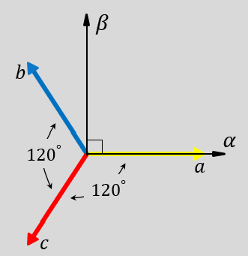
\includegraphics[width=0.5\textwidth]{Figures/5.4.1.png}
    \caption{Clark transformation.}
    \label{clark transformation}
\end{figure}
\begin{figure}[H]
    \centering
    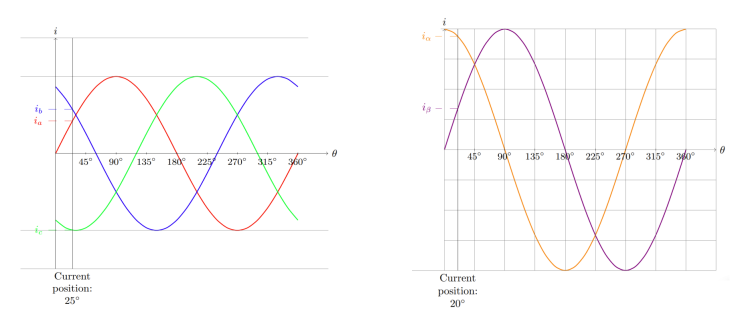
\includegraphics[width=1.1\textwidth]{Figures/5.4.2.png}
    \caption{Clark transformation waveform.}
    \label{clark transformation graph}
\end{figure}

\begin{center}
        \begin{equation*}
            \left[\begin{array}{c}
                v_\alpha \\[6pt]
                v_\beta \\[6pt]
                v_0
            \end{array}\right]
            = \frac{2}{3}
            \left[\begin{array}{ccc}
                1 & -\dfrac{1}{2} & -\dfrac{1}{2} \\[10pt]
                0 & \dfrac{\sqrt{3}}{2} & -\dfrac{\sqrt{3}}{2} \\[10pt]
                \dfrac{1}{2} & \dfrac{1}{2} & \dfrac{1}{2}
            \end{array}\right]
            \left[\begin{array}{c}
                v_a \\[6pt]
                v_b \\[6pt]
                v_c
            \end{array}\right]
        \end{equation*}
\end{center}
\newpage
\subsection{Park Transformation}
\begin{itemize}
    \item \textbf{Park Transform}, also known as d-q transformation.
    \item \textbf{Park} transforms \textbf{variable three-phase} ac ($a,b,c$) in \textbf{stationary frame} to \textbf{constant two-phase} ac ($d,q$) \textbf{in in rotating frame}.
\end{itemize}
\begin{figure}[H]
    \centering
    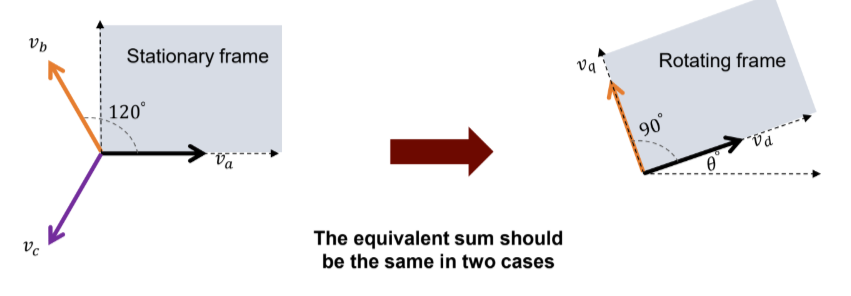
\includegraphics[width=1.1\textwidth]{Figures/5.4.3.png}
    \caption{Park transformation.}
    \label{park transformation graph}
\end{figure}

\begin{equation}
    \left[\begin{array}{c}
        v_d \\[6pt]
        v_q
    \end{array}\right]
    =
    \left[\begin{array}{cc}
        \cos(\theta)  & \sin(\theta) \\[6pt]
        -\sin(\theta) & \cos(\theta)
    \end{array}\right]
    \left[\begin{array}{c}
        v_\alpha \\[6pt]
        v_\beta
    \end{array}\right]
\end{equation}

\subsection{Park Clark Transformation}
\begin{equation}
    \left[\begin{array}{c}
        v_d \\[6pt]
        v_q
    \end{array}\right]
    =
    \frac{2}{3}
    \left[\begin{array}{ccc}
        \cos(\theta)  & \cos\!\left(\theta - \dfrac{2\pi}{3}\right) & \cos\!\left(\theta + \dfrac{2\pi}{3}\right) \\[14pt]
        \sin(\theta)  & \sin\!\left(\theta - \dfrac{2\pi}{3}\right) & \sin\!\left(\theta + \dfrac{2\pi}{3}\right)
    \end{array}\right]
    \left[\begin{array}{c}
        v_a \\[6pt]
        v_b \\[6pt]
        v_c
    \end{array}\right]
\end{equation}

\subsection{PLL(phase locked loop)}
In grid-tied power electronic interfaces—such as the three-phase static inverter topology connected to a photovoltaic (PV) array—precise synchronization with the local utility network is critical. To achieve this synchronization, a Phase-Locked Loop (PLL) is utilized as the primary control block to continuously track the utility grid's voltage vector profile. 

\begin{figure}[H]
    \centering
    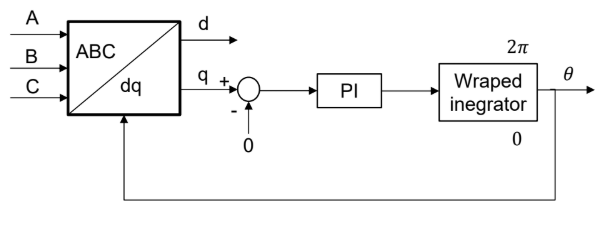
\includegraphics[width=1.1\textwidth]{Figures/5.4.4.png}
    \caption{PLL control circuit.}
    \label{PLL}
\end{figure}

\subsection{Control Circuit}
The aim is to control the converter current (act as controlled current source) to achieve certain purpose like , injecting active power (renewable sources), injecting reactive power (support grid voltage), or controlling active and reactive power (grid quality )
\begin{figure}[H]
    \centering
    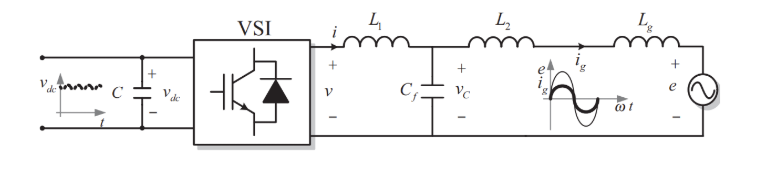
\includegraphics[width=1.1\textwidth]{Figures/5.4.20.png}
    \caption{Grid connected VSC.}
    \label{Grid connected VSC}
\end{figure}
\begin{figure}[H]
    \centering
    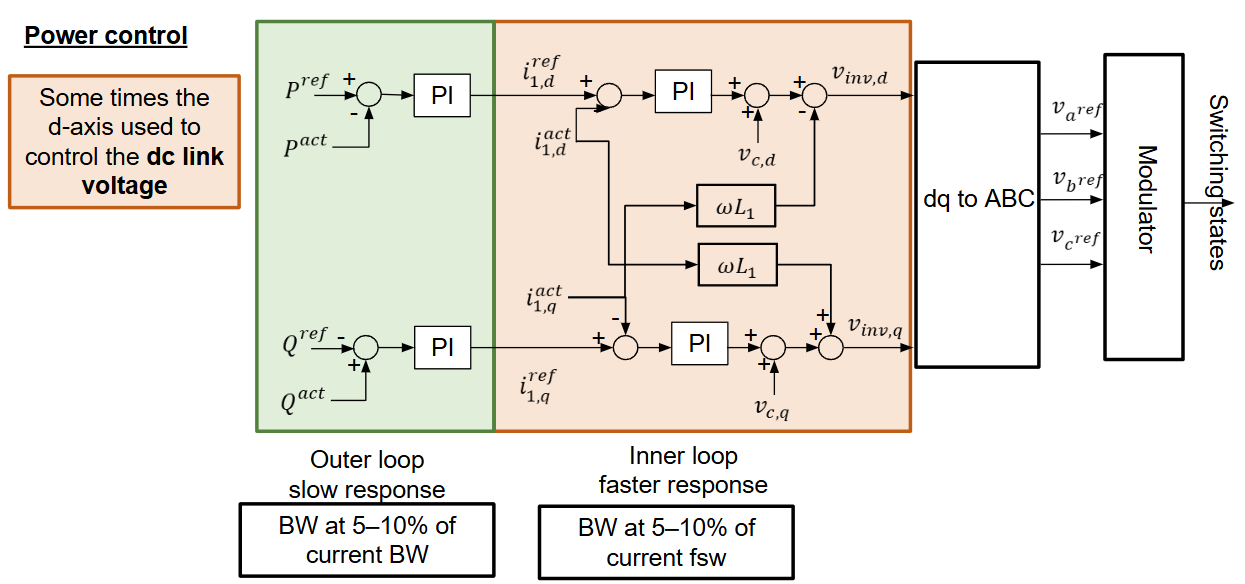
\includegraphics[width=1.1\textwidth]{Figures/5.4.21.png}
    \caption{Control diagram.}
    \label{control diagram.}
\end{figure}

% ==========================================================
% SECTION: ACTIVE AND REACTIVE POWER IN THE dq FRAME
% ==========================================================

\subsection{Active and Reactive Power Modeling in the Synchronous $d\text{-}q$ Frame}

In a three-phase system, the instantaneous active power ($P$) and reactive power ($Q$) can be expressed directly using the orthogonal components of the synchronous rotating $d\text{-}q$ reference frame. Using the amplitude-invariant transformation convention, the comprehensive power expressions are defined as follows:

\begin{equation}
    P = \frac{3}{2} \left( v_d i_d + v_q i_q \right)
\end{equation}

\begin{equation}
    Q = \frac{3}{2} \left( v_q i_d - v_d i_q \right)
\end{equation}

Where $v_d, v_q$ represent the $d\text{-}q$ axis voltage components, and $i_d, i_q$ represent the corresponding $d\text{-}q$ axis current vectors injected into the grid interface.
\newpage
\subsubsection{ Power Control}

for balanced three phase voltage aligned with grid:
\begin{equation}
    v_q = 0
\end{equation}

Substituting $v_q = 0$ into the core power equations simplifies the expressions, yielding a highly desirable decoupled relationship:

\begin{equation}
    P = \frac{3}{2} v_d i_d \quad \longrightarrow \quad \text{Controlled directly via } i_d
\end{equation}

\begin{equation}
    Q = -\frac{3}{2} v_d i_q \quad \longrightarrow \quad \text{Controlled directly via } i_q
\end{equation}

\paragraph{Control Implications}
This mathematical simplification provides a foundational advantage for grid-tied inverter operation:
\begin{itemize}
    \item \textbf{Active Power Regulation ($P$):} Because the grid voltage $v_d$ is regulated to a constant value by the utility infrastructure, the instantaneous active power transfer becomes purely dependent on the direct-axis current component ($i_d$).
    \item \textbf{Reactive Power Regulation ($Q$):} Similarly, the instantaneous reactive power flow becomes decoupled and depends solely on adjusting the quadrature-axis current component ($i_q$). 
\end{itemize}
Consequently, the system can implement separate, independent PI tracking regulators for $i_d$ and $i_q$, allowing for concurrent optimization of active power extraction (e.g., maximizing PV output) and reactive power mitigation (achieving unity power factor or supporting grid voltage stability).

\subsection{Simulation of Inverter}
The goal is that the active power = 50000W , so Id = 100A

Note: The dc link must be more than phase to phase voltage at least double
\begin{figure}[H]
    \centering
    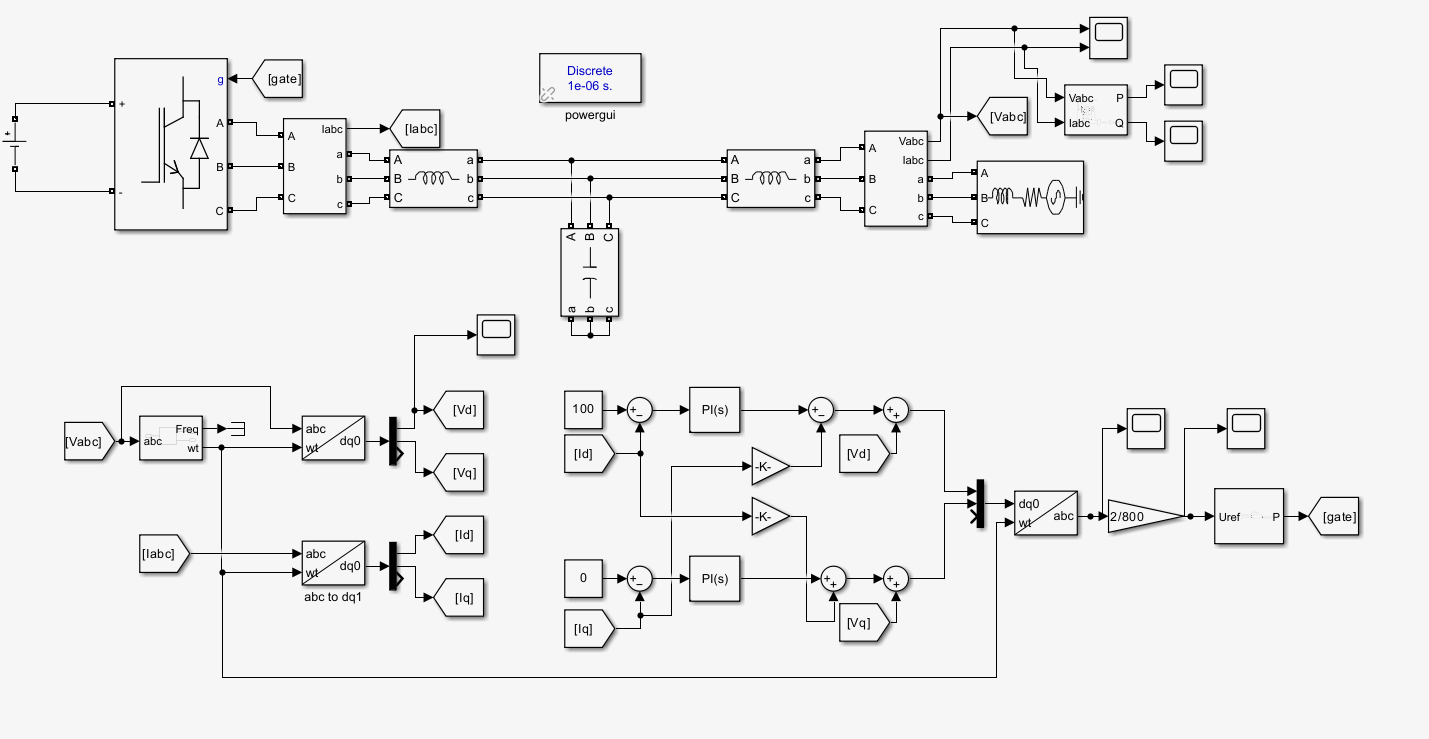
\includegraphics[width=1.1\textwidth]{Figures/5.4.5.png}
    \caption{Inverter tied with grid.}
    \label{inverter tied with grid}
\end{figure}
\subsubsection{Results}
Ma is less than 1
\begin{figure}[H]
    \centering
    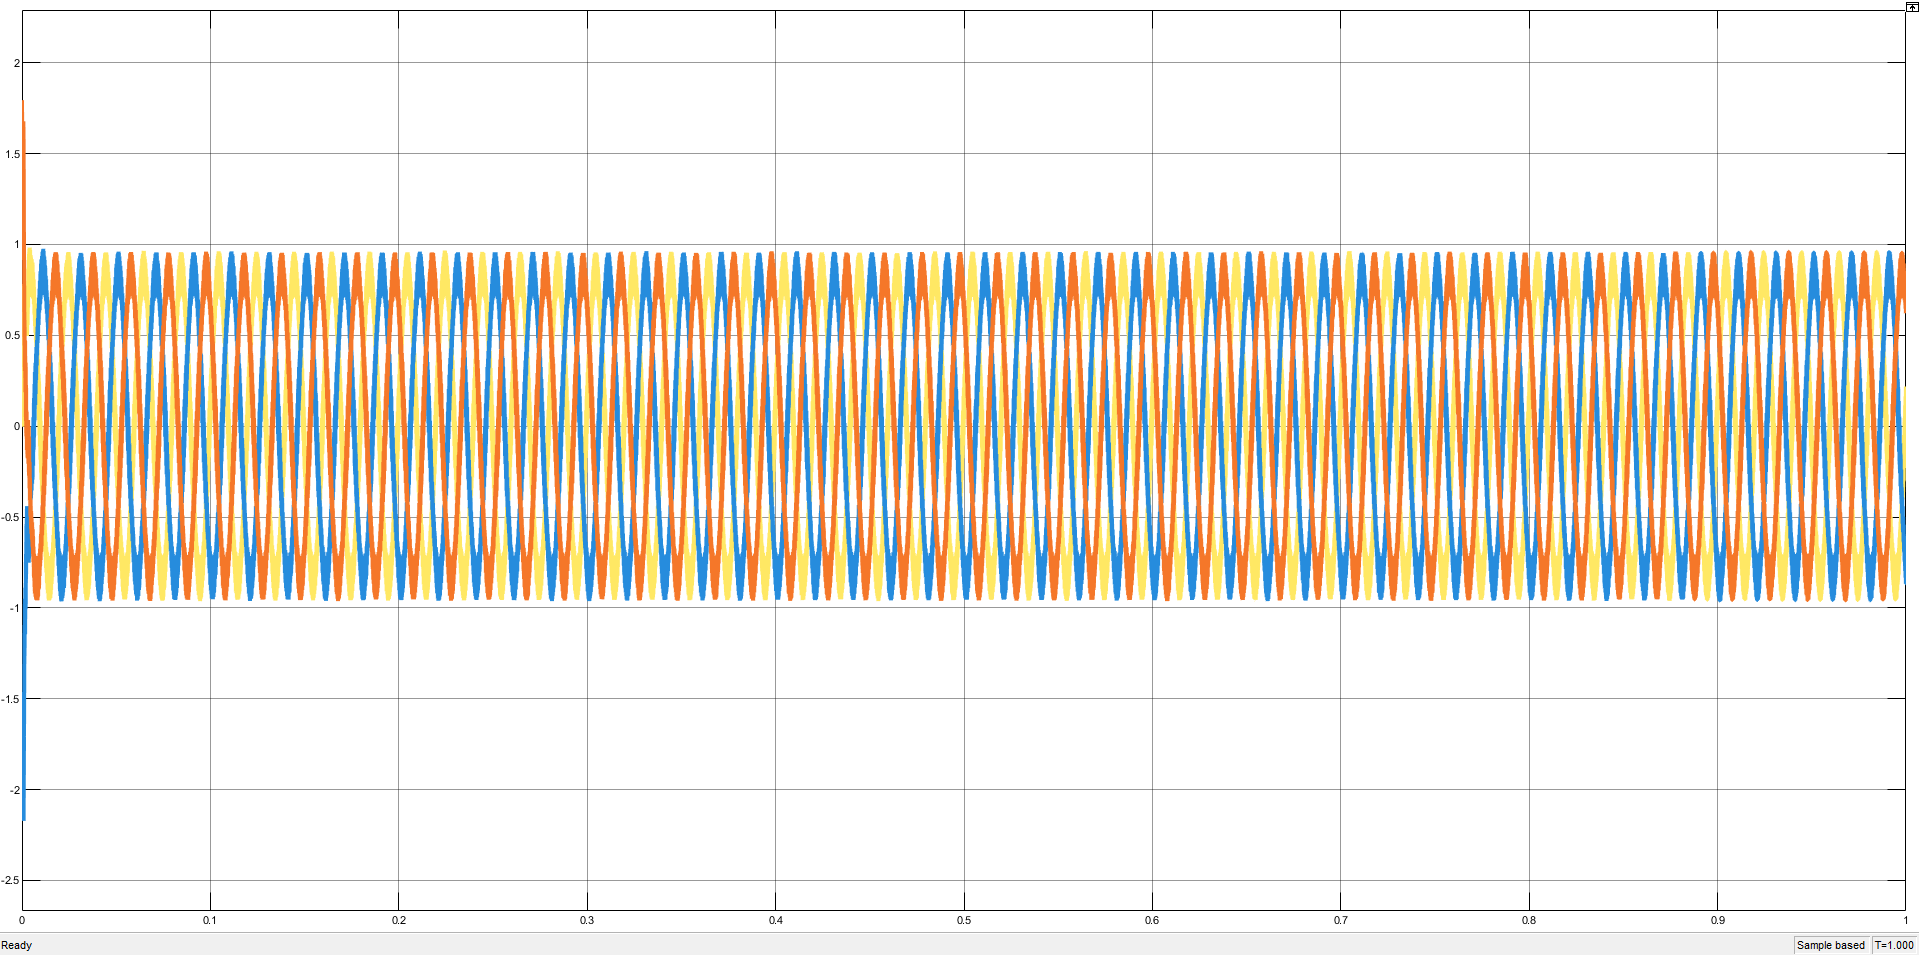
\includegraphics[width=1.1\textwidth]{Figures/5.4.6.png}
    \caption{Modulation index.}
    \label{modulation index}
\end{figure}
\begin{figure}[H]
    \centering
    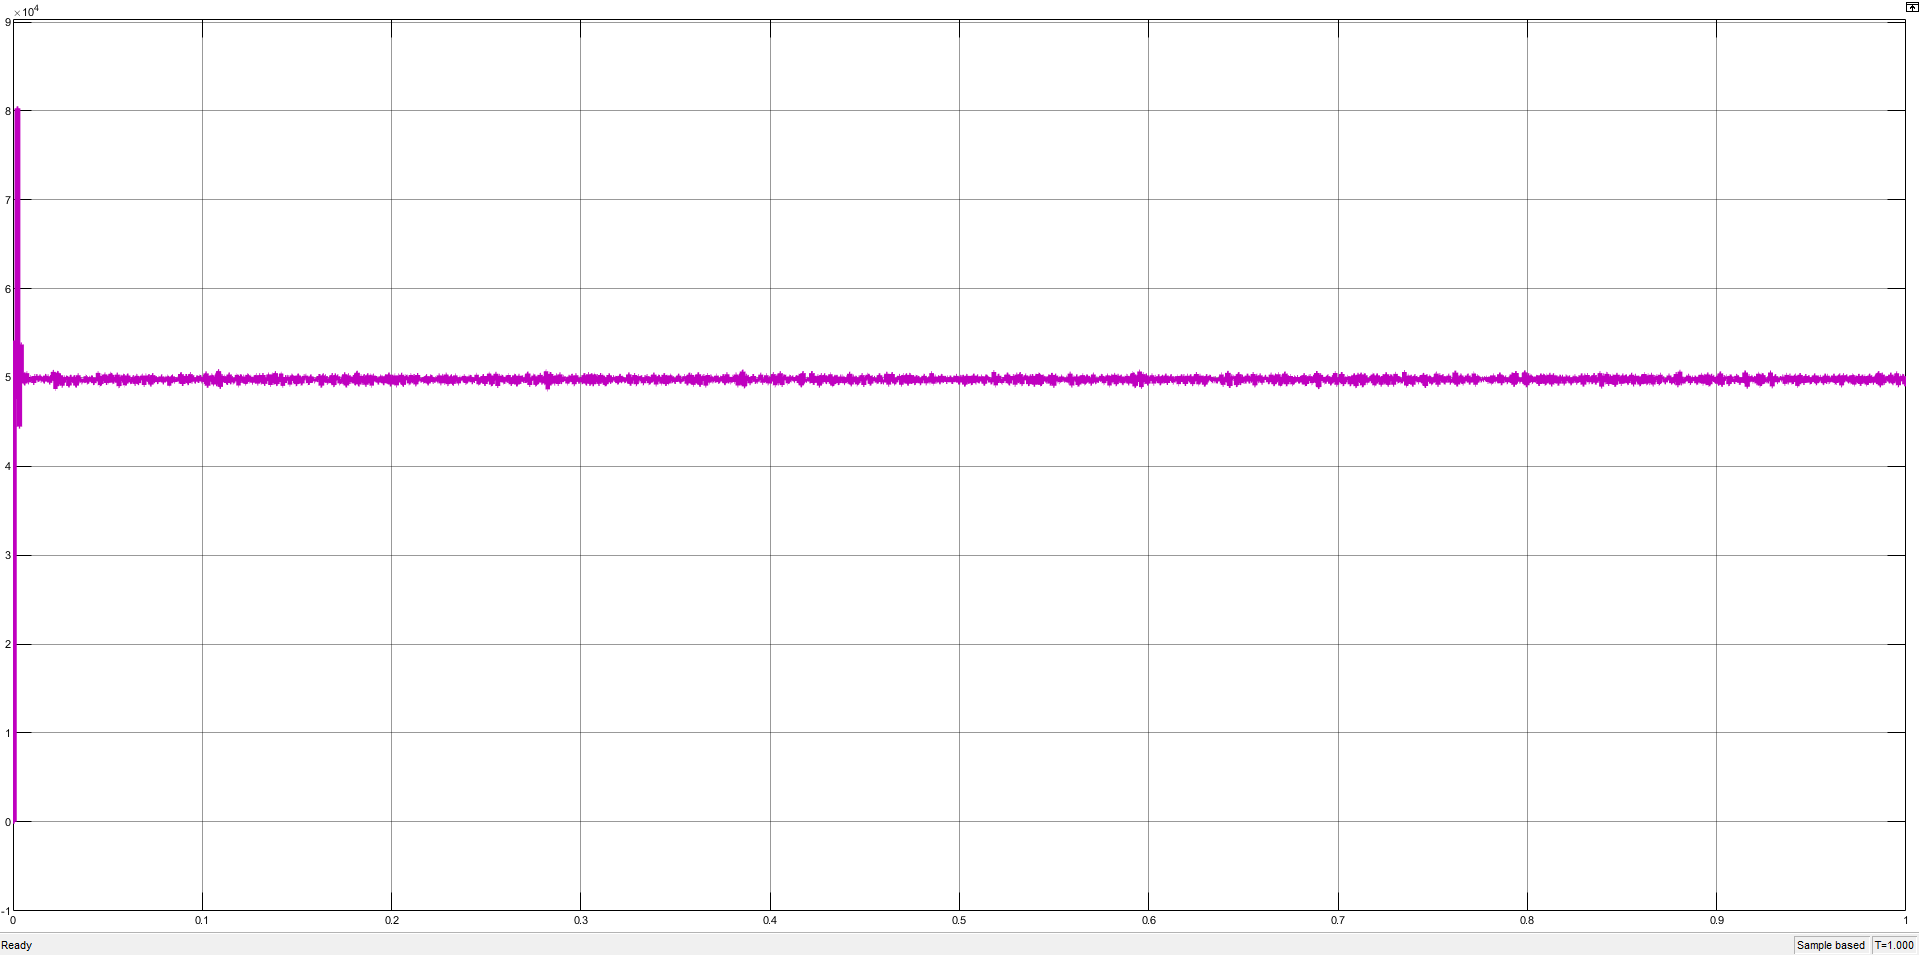
\includegraphics[width=1.1\textwidth]{Figures/5.4.7.png}
    \caption{Grid power.}
    \label{grid power}
\end{figure}

\subsection{Simulation of PV System with Interleaved Boost Tied with Grid}
now the dc link is maintained at 800V as the phase to phase voltage of the grid is 400V
\begin{figure}[H]
    \centering
    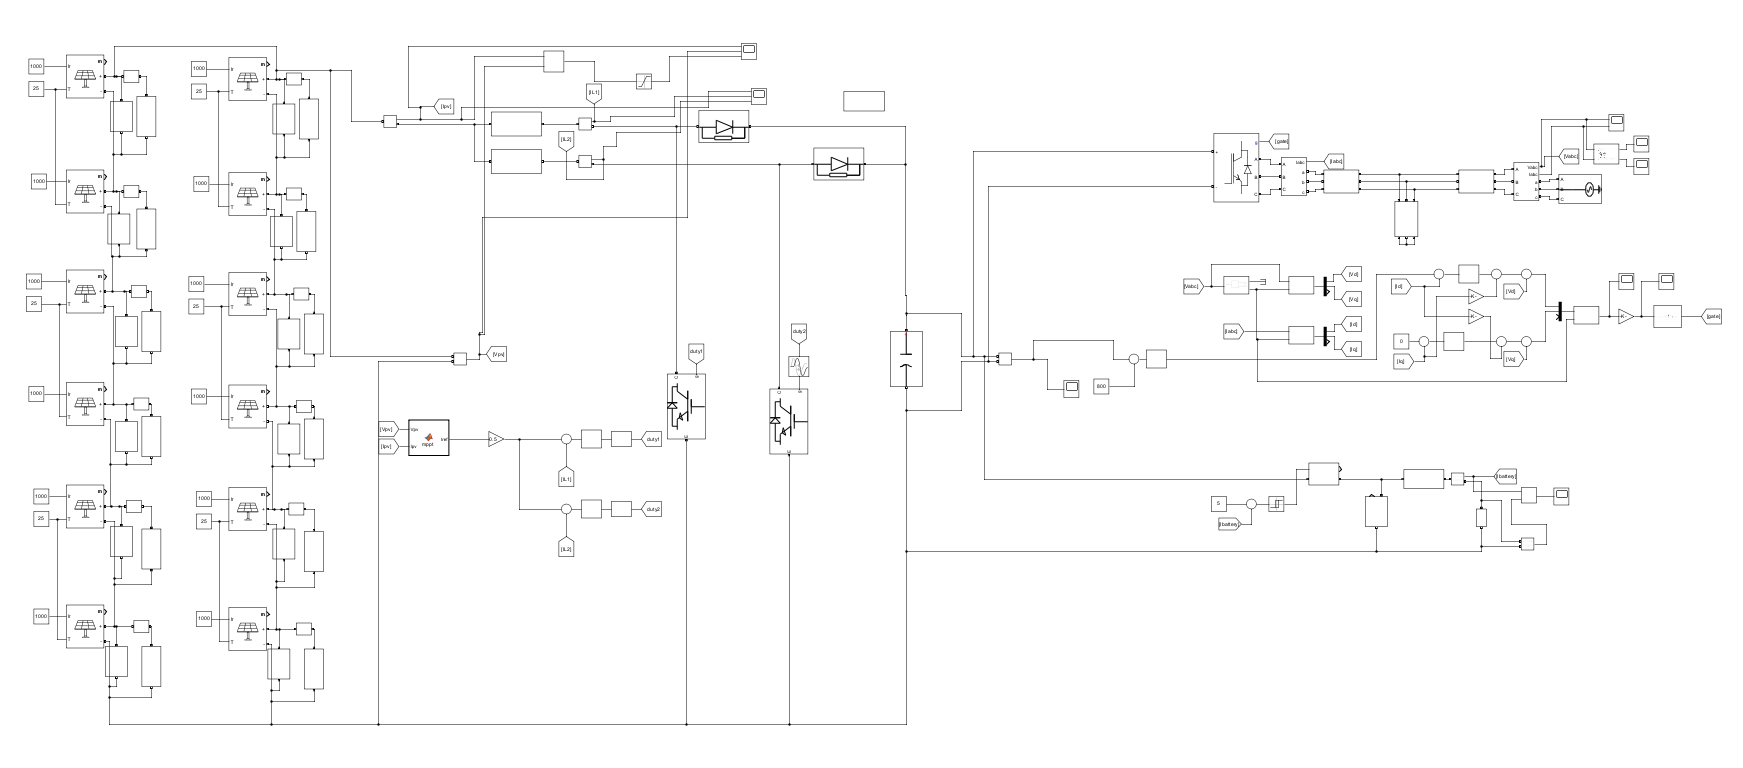
\includegraphics[width=1.1\textwidth]{Figures/5.4.8.png}
    \caption{Grid power.}
    \label{grid power}
\end{figure}

\subsubsection{Results if Ibattery = 10A}
\noindent
\begin{minipage}[t]{0.5\textwidth}
\vspace{0pt}
\begin{itemize}
  \item As shown, current is almost $17.36 \times 2$, the input voltage is also aligned
        with design calculations and output power is 8476\,W, ideally should be 8520\,W,
        but there are switching losses and conduction losses (diodes have forward voltage,
        etc.).

  \item now the dc link is maintained at 800V as the phase to phase voltage of the grid is 400V

  \item Ripples of inductor current $= 35.38 - 34.78 = 0.6$\,A.
  \item as Ibattery = 10A so dc link will send the rest power to the grid.
\end{itemize}
\end{minipage}
\hfill
\begin{minipage}[t]{0.4\textwidth}
\vspace{0pt}
  \centering
  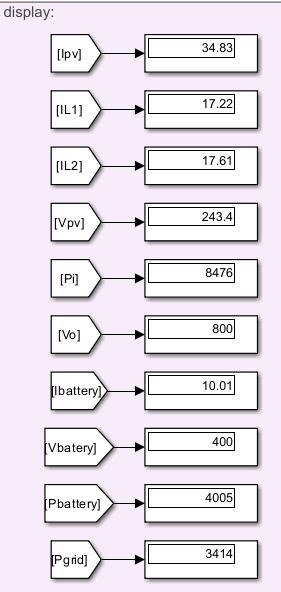
\includegraphics[width=\textwidth]{Figures/5.4.9.png}
  \captionof{figure}{Displays of System.}
  \label{fig:Displays of system}
\end{minipage}

\begin{figure}[H]
    \centering
    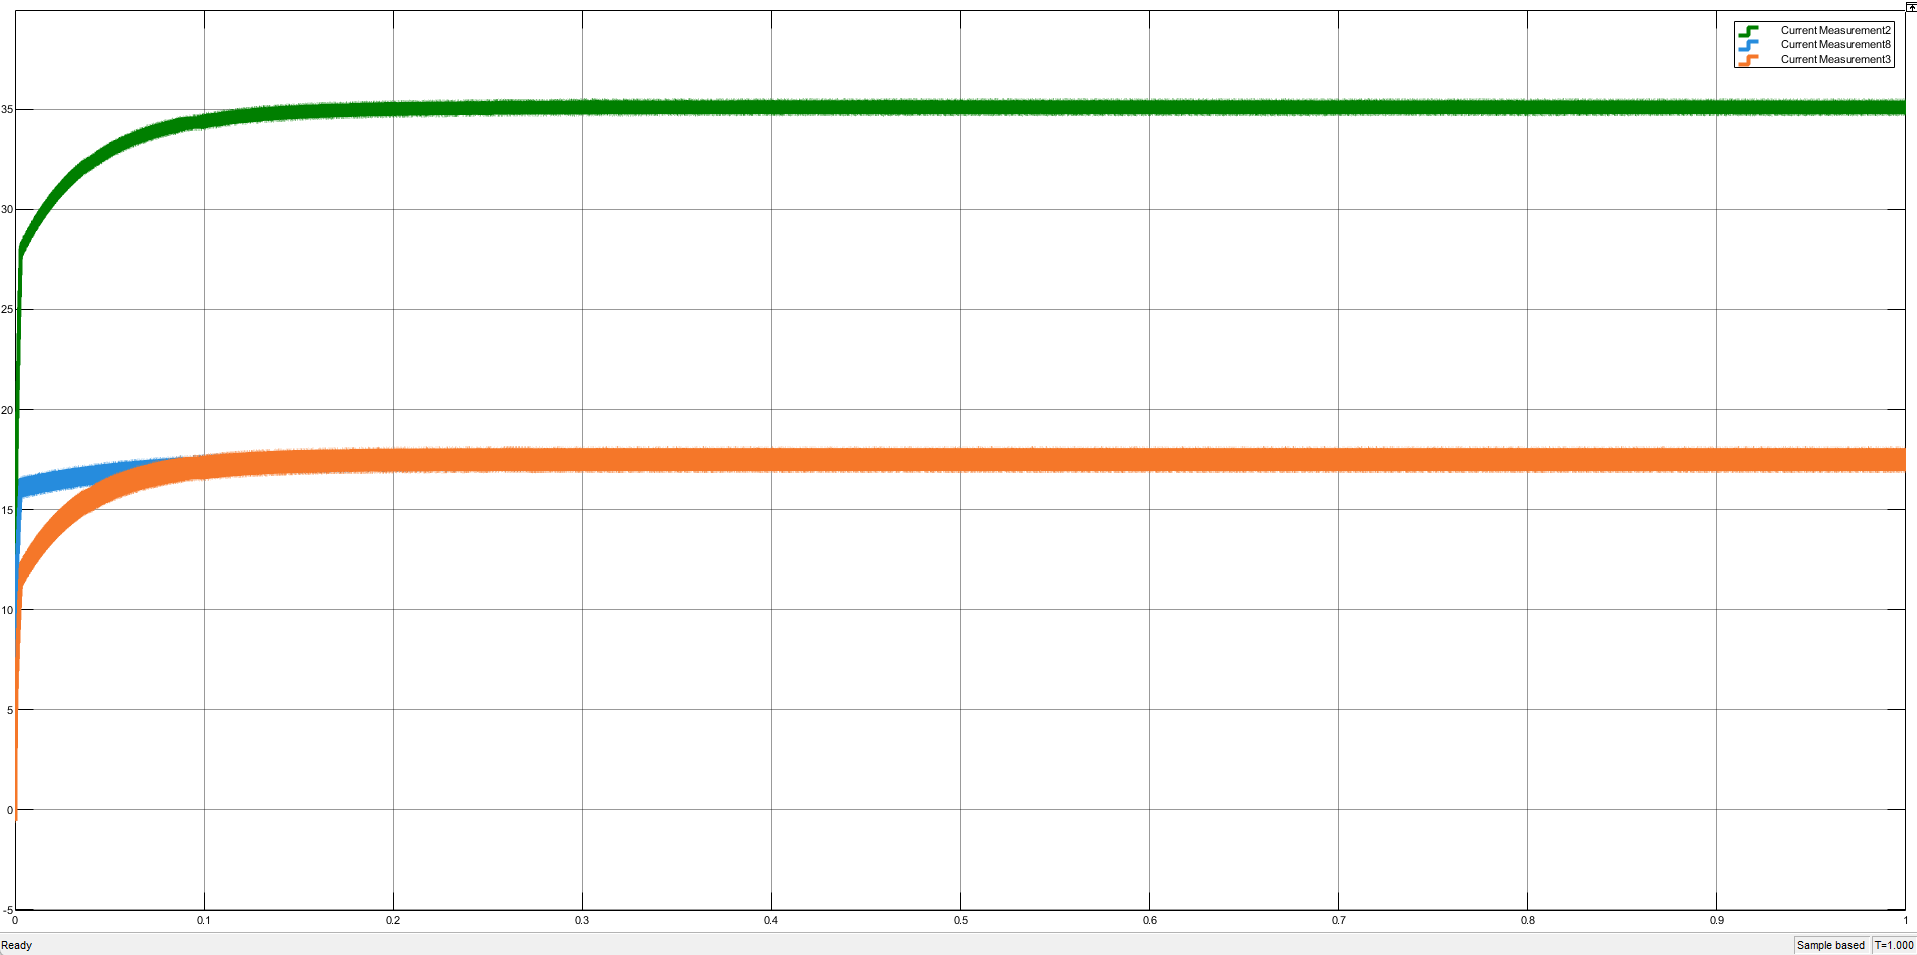
\includegraphics[width=1\textwidth]{Figures/5.4.10.png}
    \caption{Total Current, Inductor Current 1, Inductor Current 2.}
    \label{total current , inductor current 1 ,  inductor current 2 of all system}
\end{figure}

\begin{figure}[H]
    \centering
    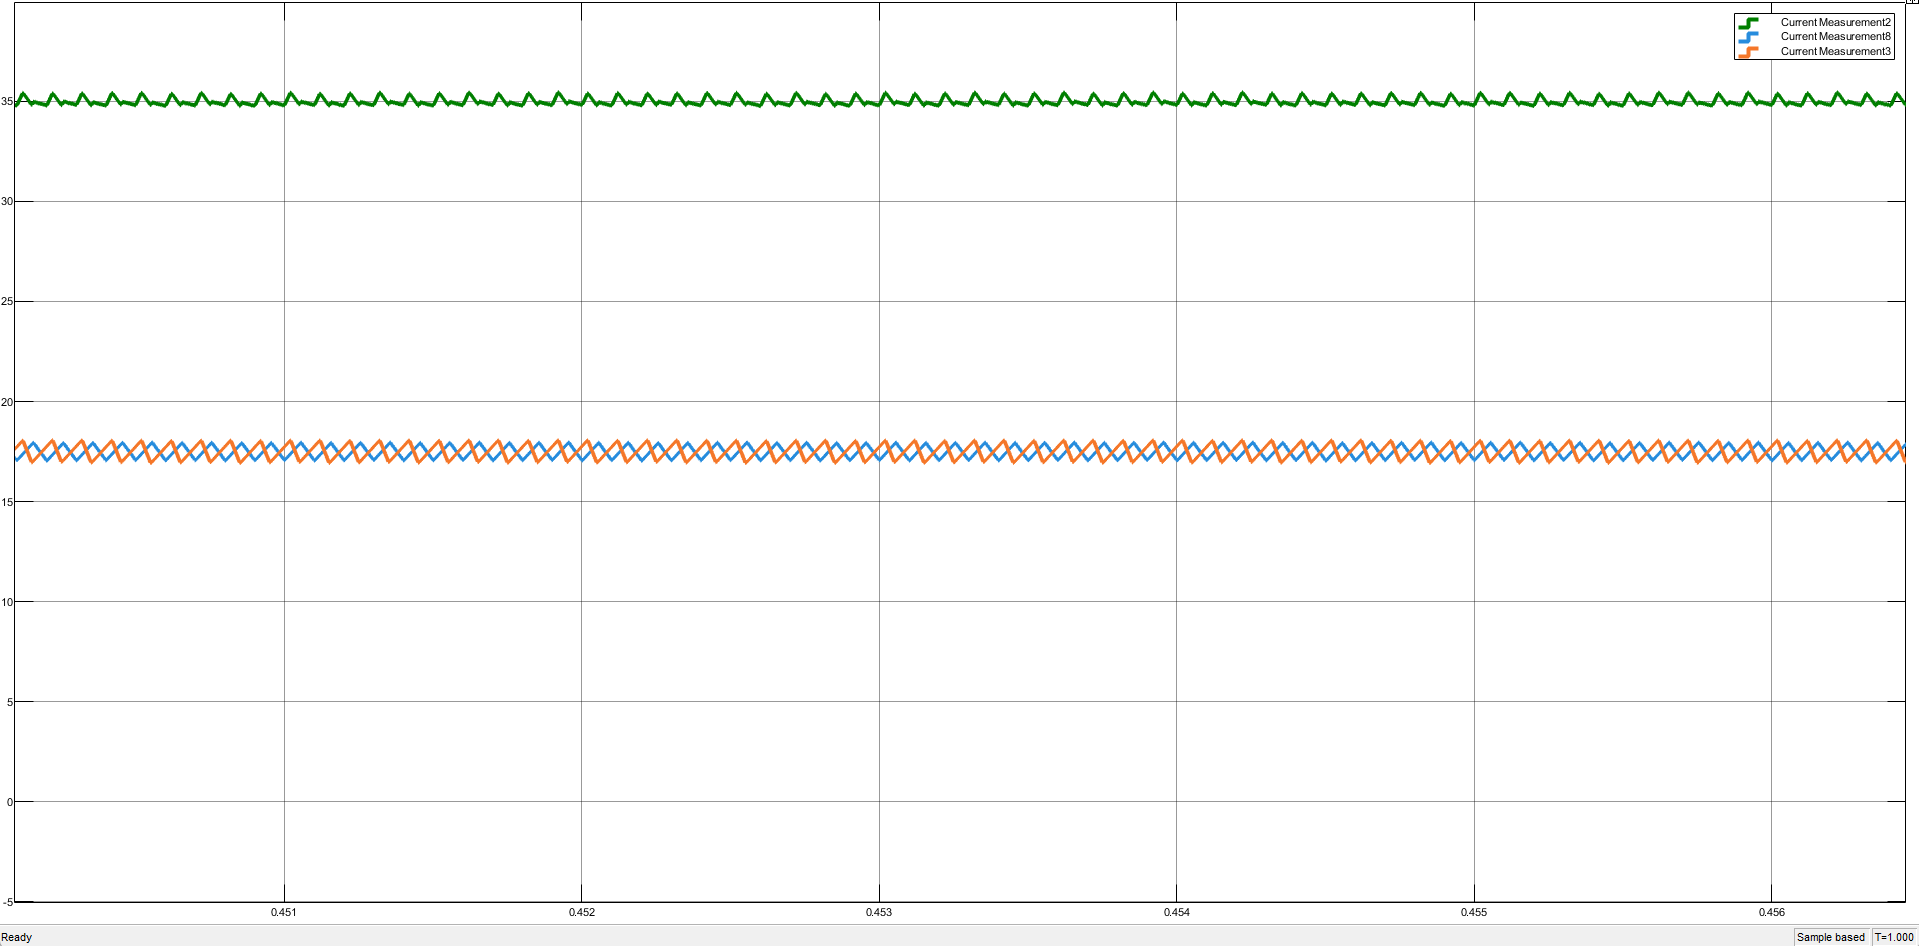
\includegraphics[width=1\textwidth]{Figures/5.4.11.png}
    \caption{Total Current, Inductor Current 1, Inductor Current 2.}
    \label{total current , inductor current 1 ,  inductor current 2 zoom of all system}
\end{figure}

\begin{figure}[H]
    \centering
    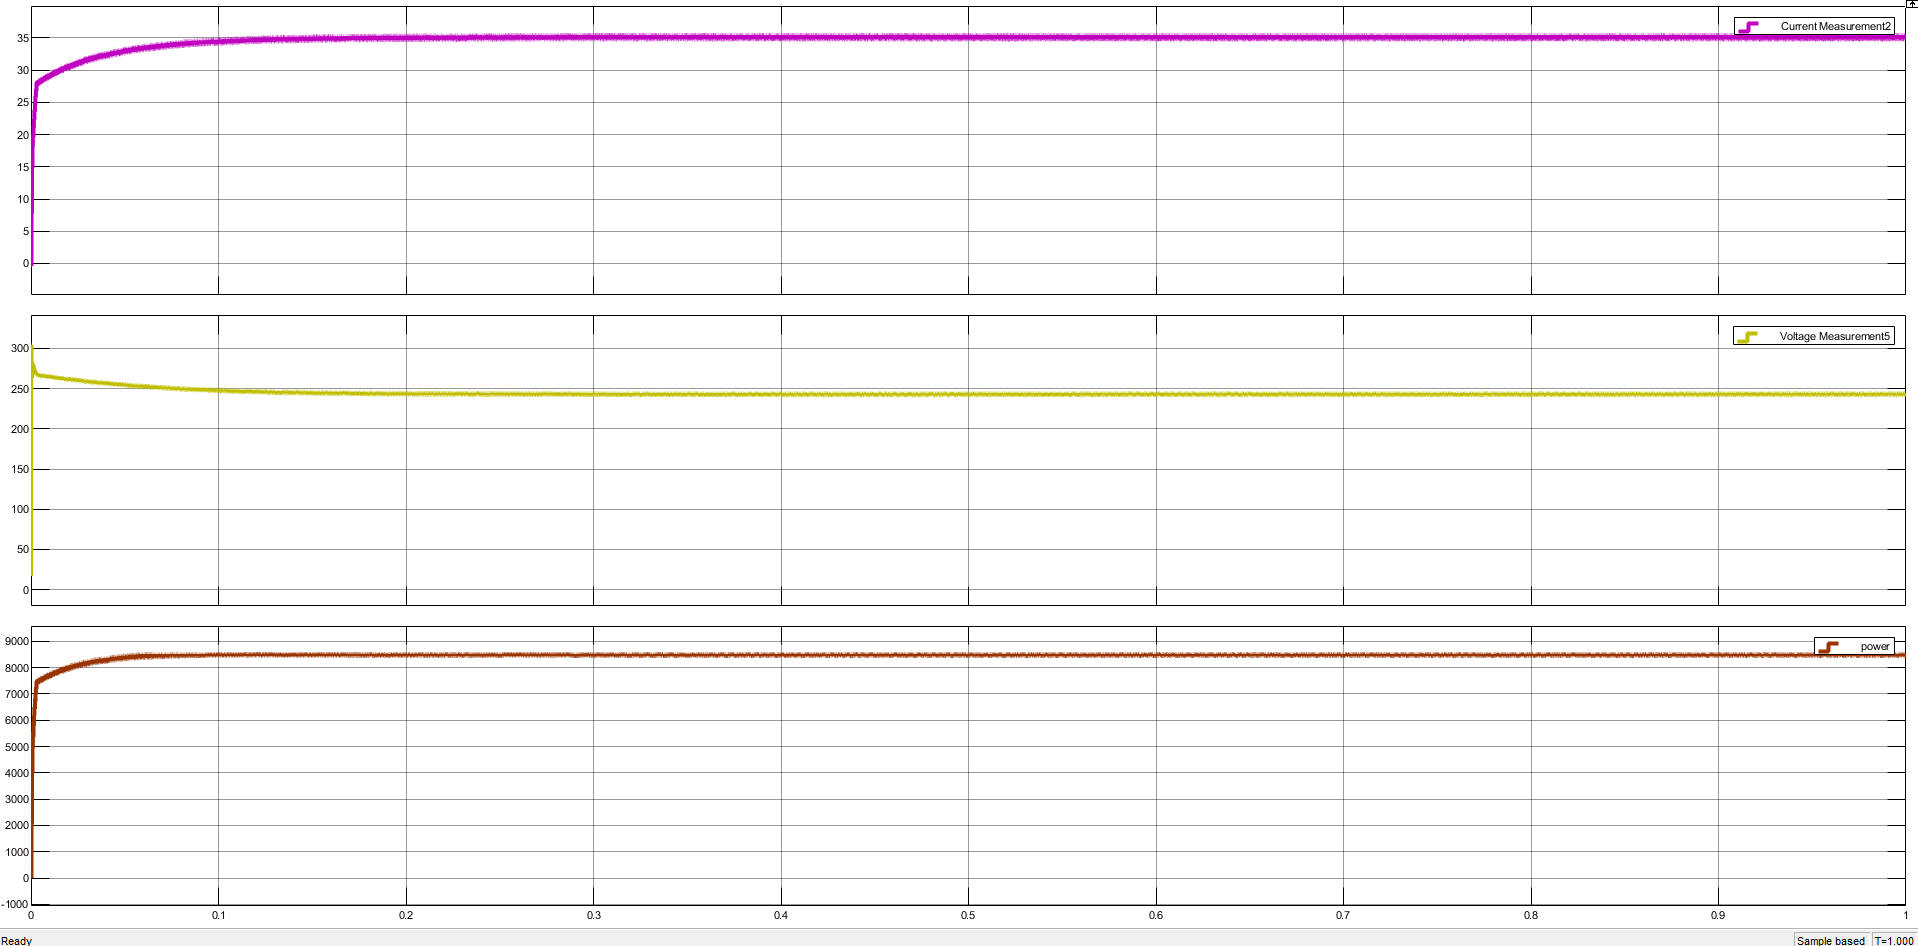
\includegraphics[width=1\textwidth]{Figures/5.4.12.png}
    \caption{Input Current, Voltage, Power.}
    \label{input current , voltage , power. of all system}
\end{figure}

\begin{figure}[H]
    \centering
    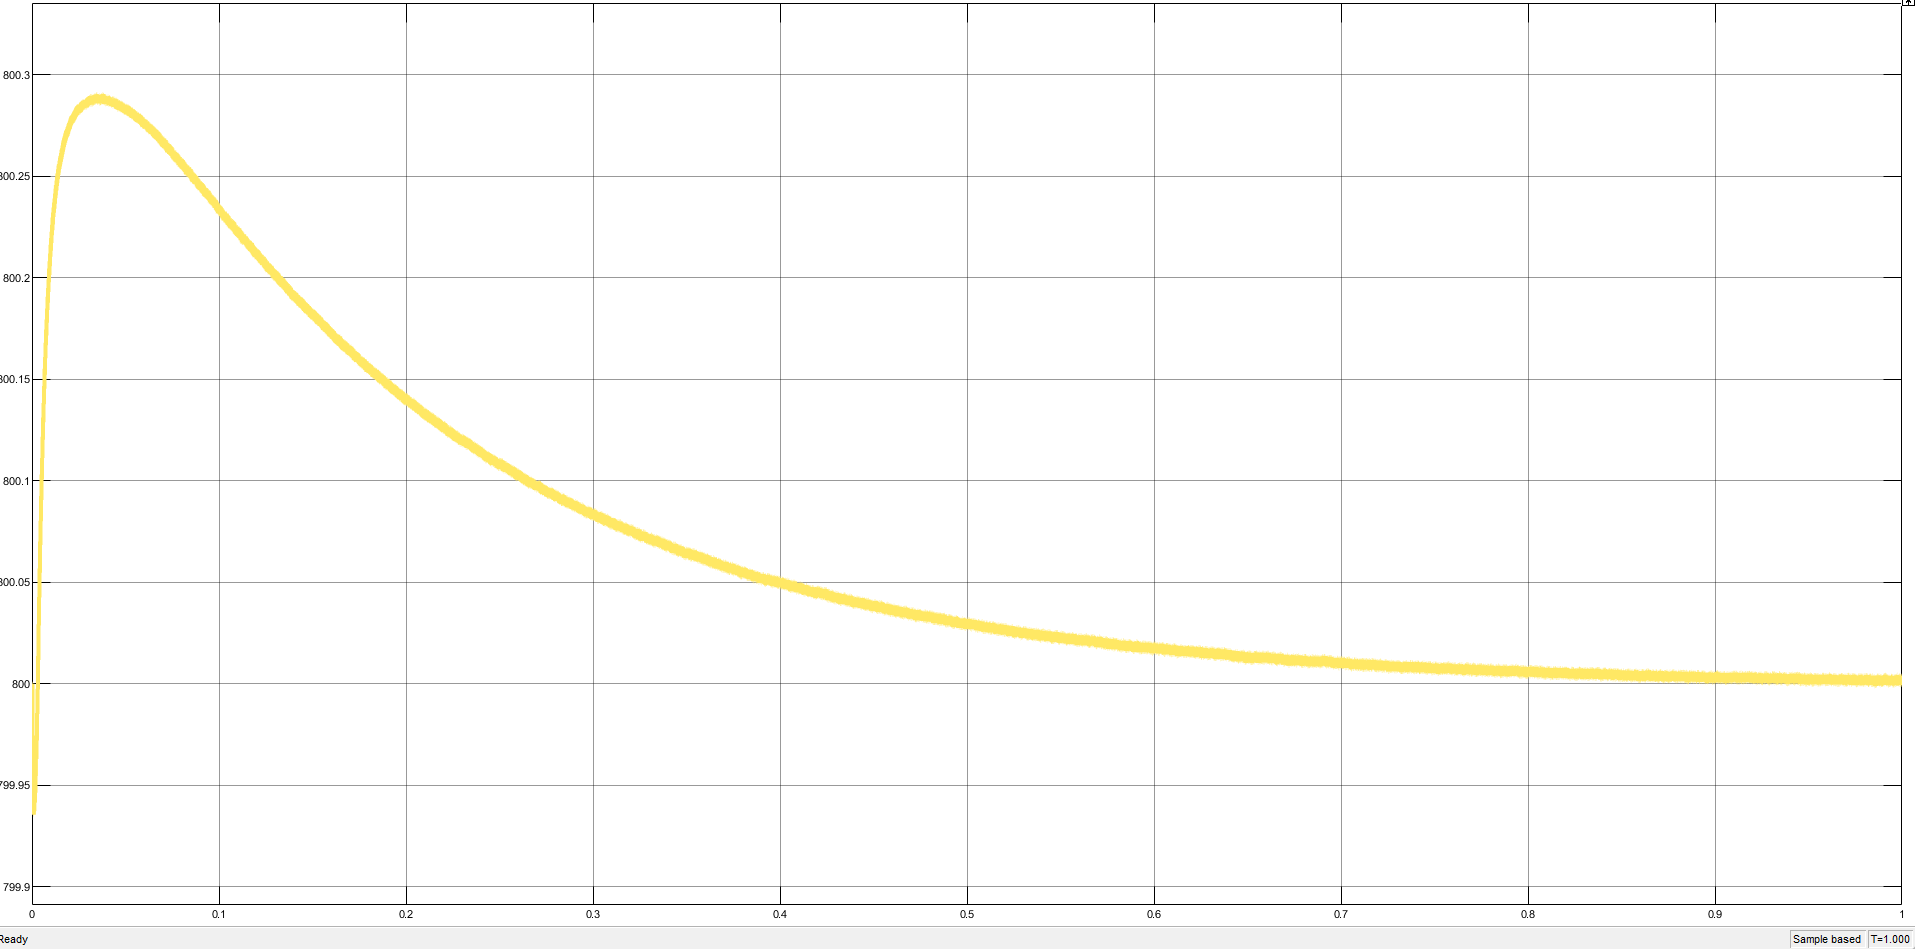
\includegraphics[width=1\textwidth]{Figures/5.4.13.png}
    \caption{Output Voltage.}
    \label{Output voltage of all system}
\end{figure}

\begin{figure}[H]
    \centering
    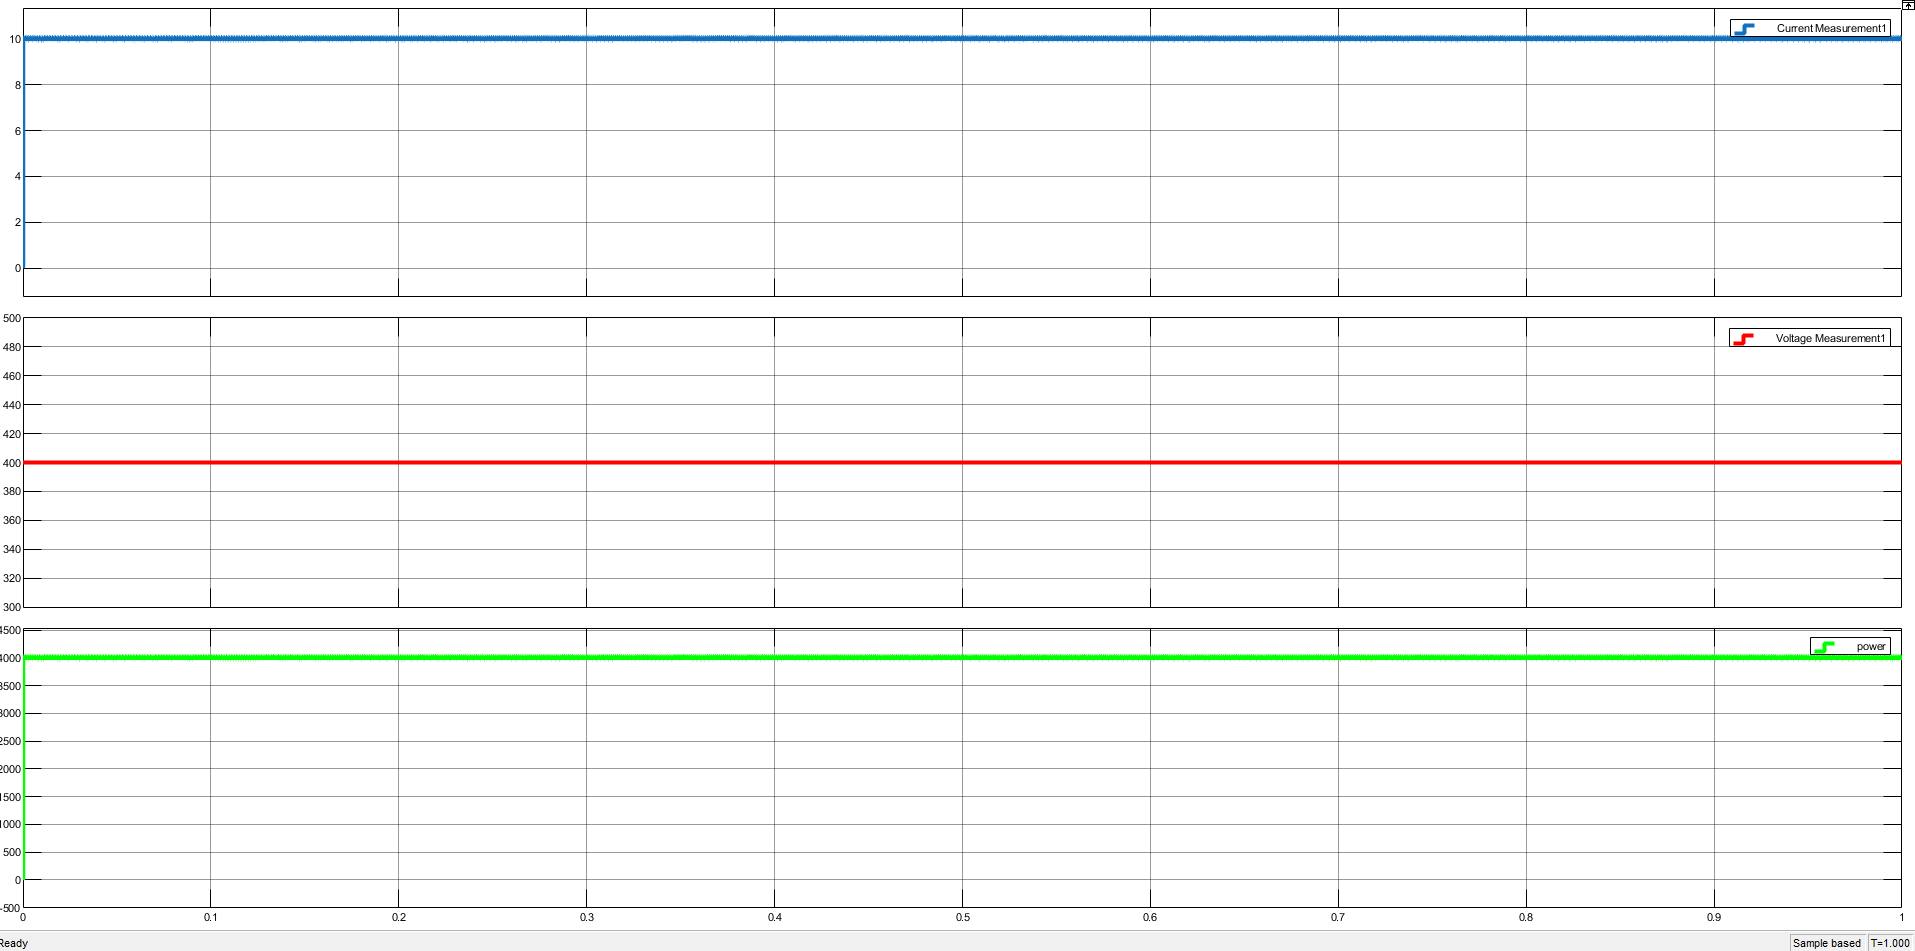
\includegraphics[width=1\textwidth]{Figures/5.4.14.png}
    \caption{Ibattery, Vbattery, Pbattery.}
    \label{Ibattery , Vbattery , Pbattery of all system}
\end{figure}

\begin{figure}[H]
    \centering
    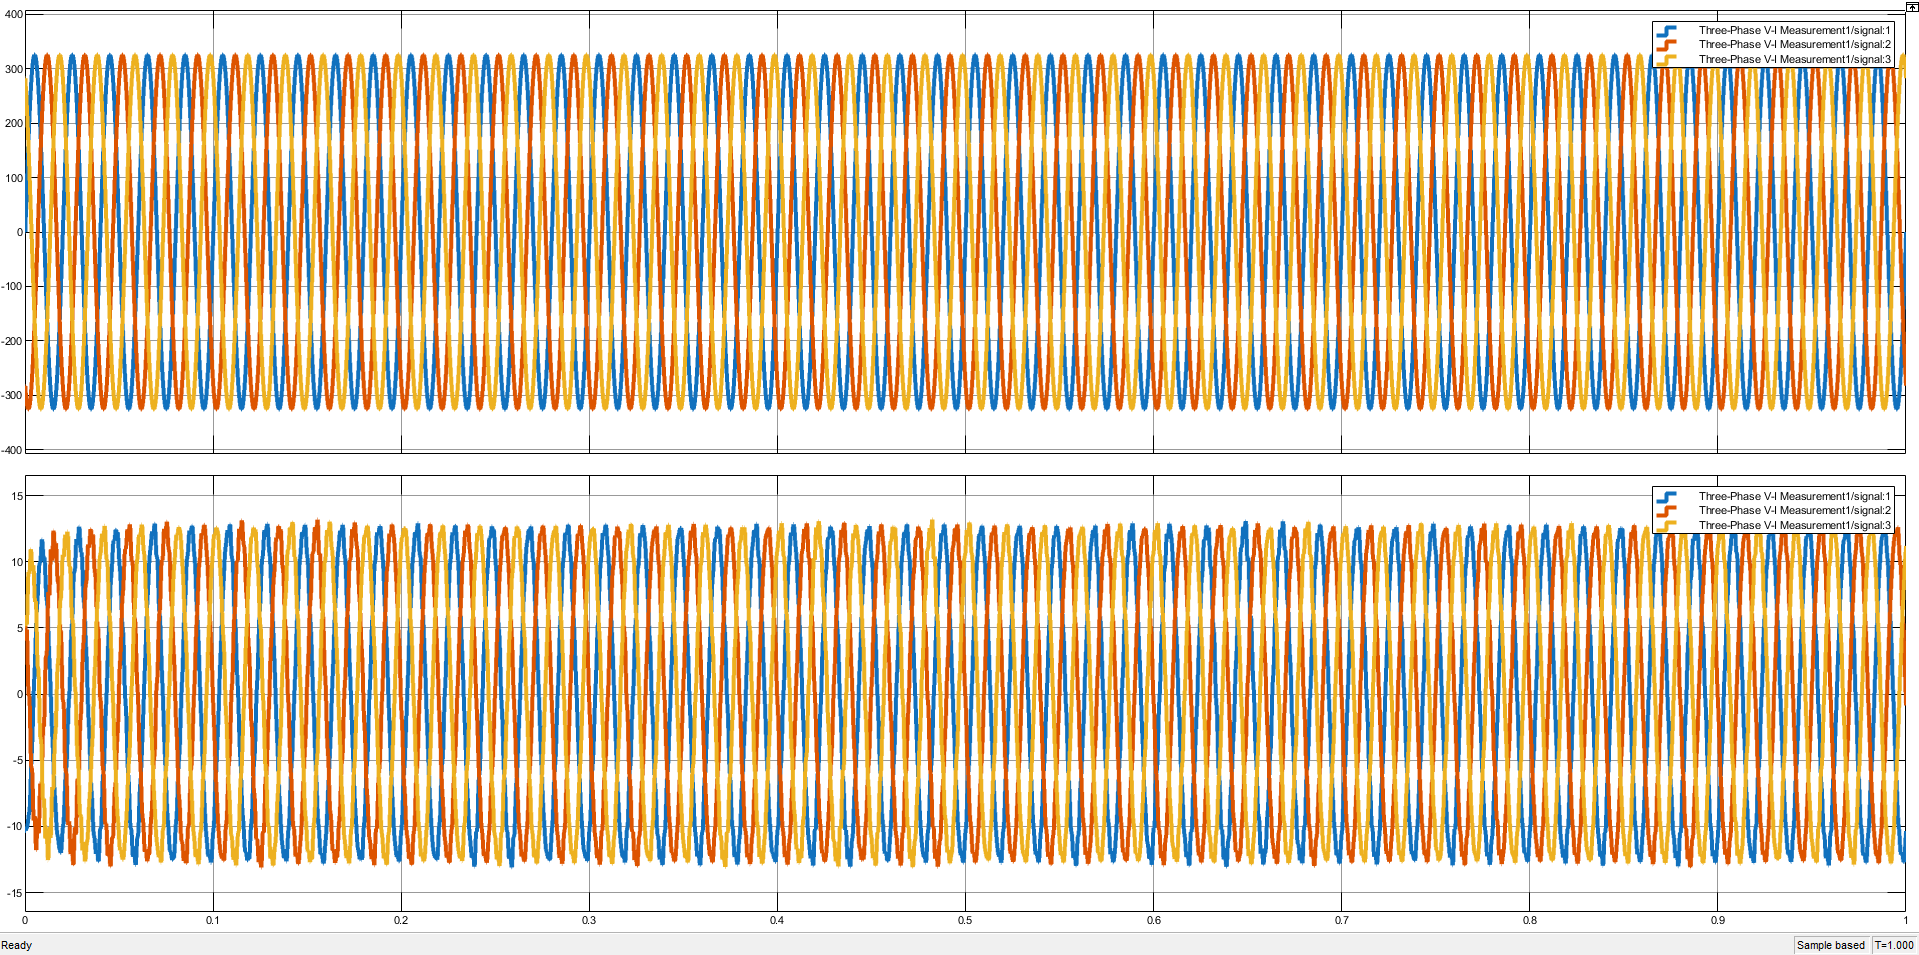
\includegraphics[width=1\textwidth]{Figures/5.4.15.png}
    \caption{3-phase Voltage, 3-phase Current.}
    \label{3-phase voltage , 3-phase current}
\end{figure}

\begin{figure}[H]
    \centering
    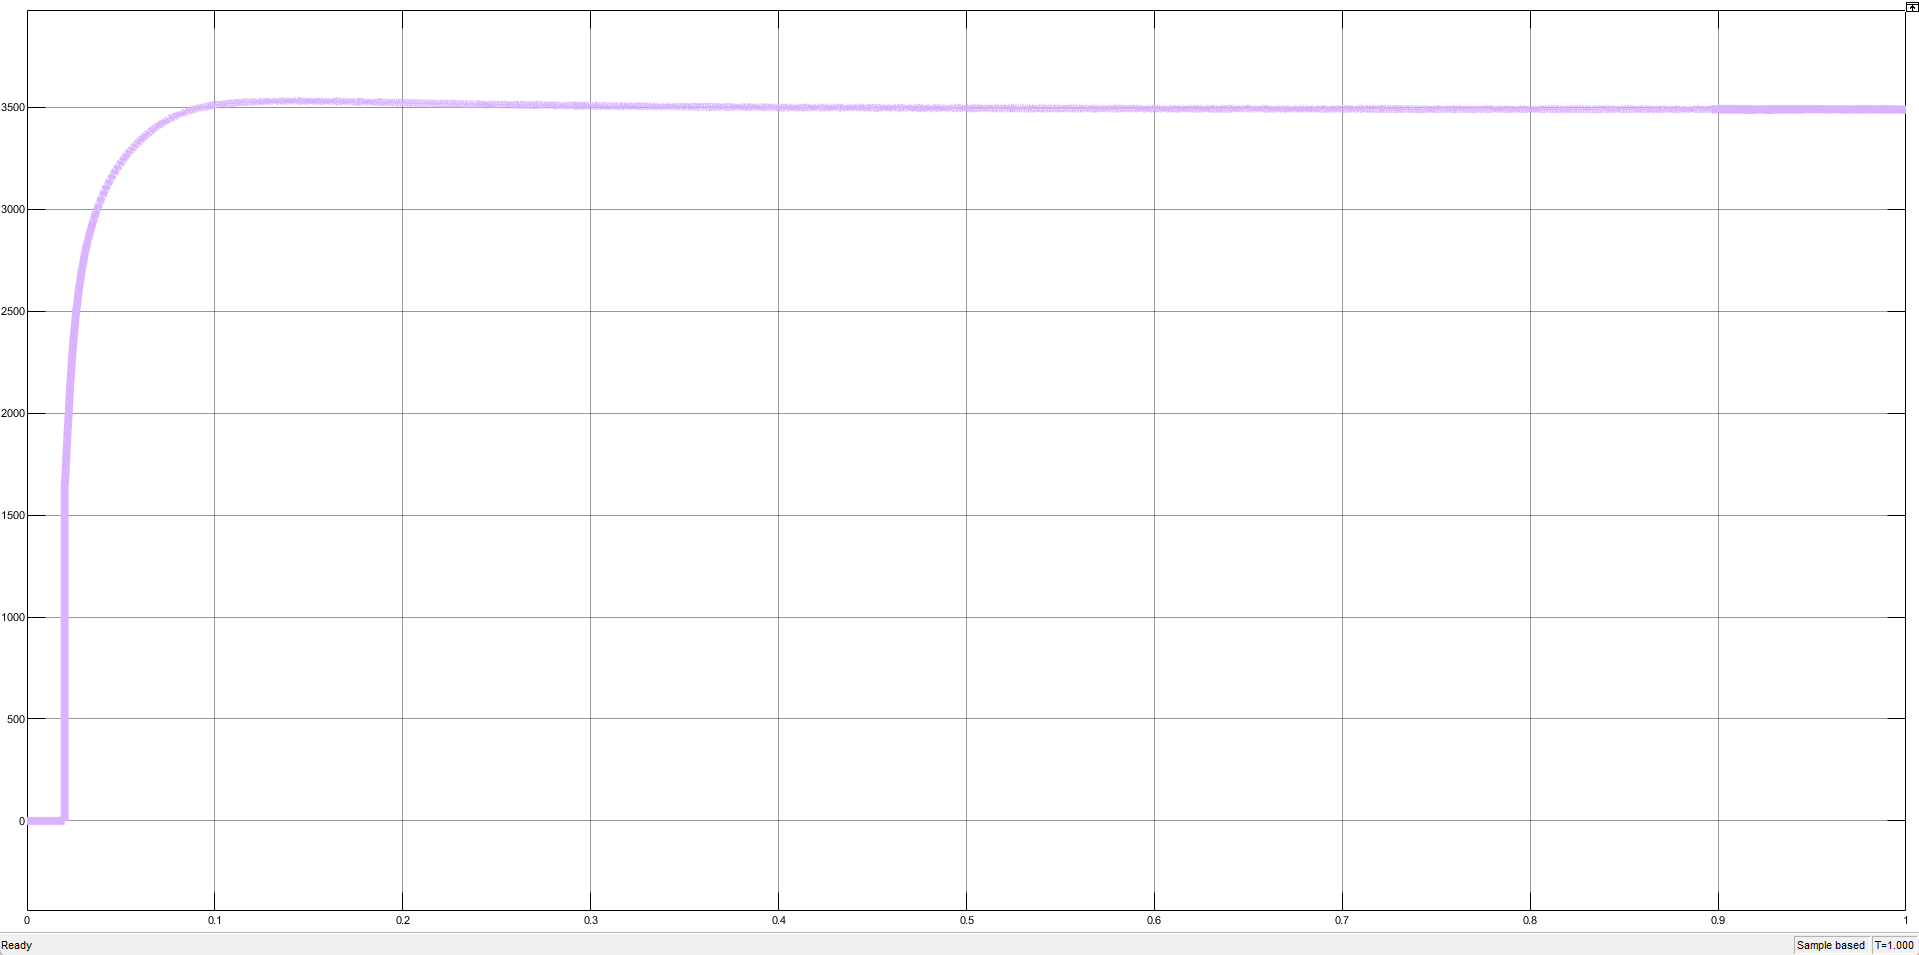
\includegraphics[width=1\textwidth]{Figures/5.4.16.png}
    \caption{Grid Power.}
    \label{grid power oa the system}
\end{figure}

\subsubsection{Results if Ibattery = 30A}
\noindent
\begin{minipage}[t]{0.5\textwidth}
\vspace{0pt}
\begin{itemize}
  \item As shown, current is almost $17.36 \times 2$, the input voltage is also aligned
        with design calculations and output power is 8492\,W, ideally should be 8520\,W,
        but there are switching losses and conduction losses (diodes have forward voltage,
        etc.).

  \item now the dc link is maintained at 800V as the phase to phase voltage of the grid is 400V

  \item Ripples of inductor current $= 35.38 - 34.78 = 0.6$\,A.
  \item as Ibattery = 30A so dc link will Receive the rest power from the grid so EV can be fully chargred.
   \item the rest graphs will be the same as case 1.
\end{itemize}
\end{minipage}
\hfill
\begin{minipage}[t]{0.4\textwidth}
\vspace{0pt}
  \centering
  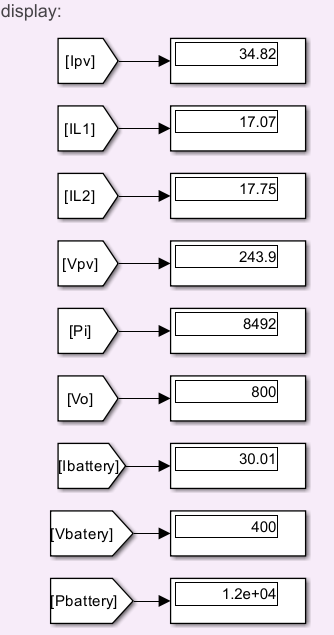
\includegraphics[width=\textwidth]{Figures/5.4.17.png}
  \captionof{figure}{Displays of system.}
  \label{fig:Displays of system2}
\end{minipage}

\begin{figure}[H]
    \centering
    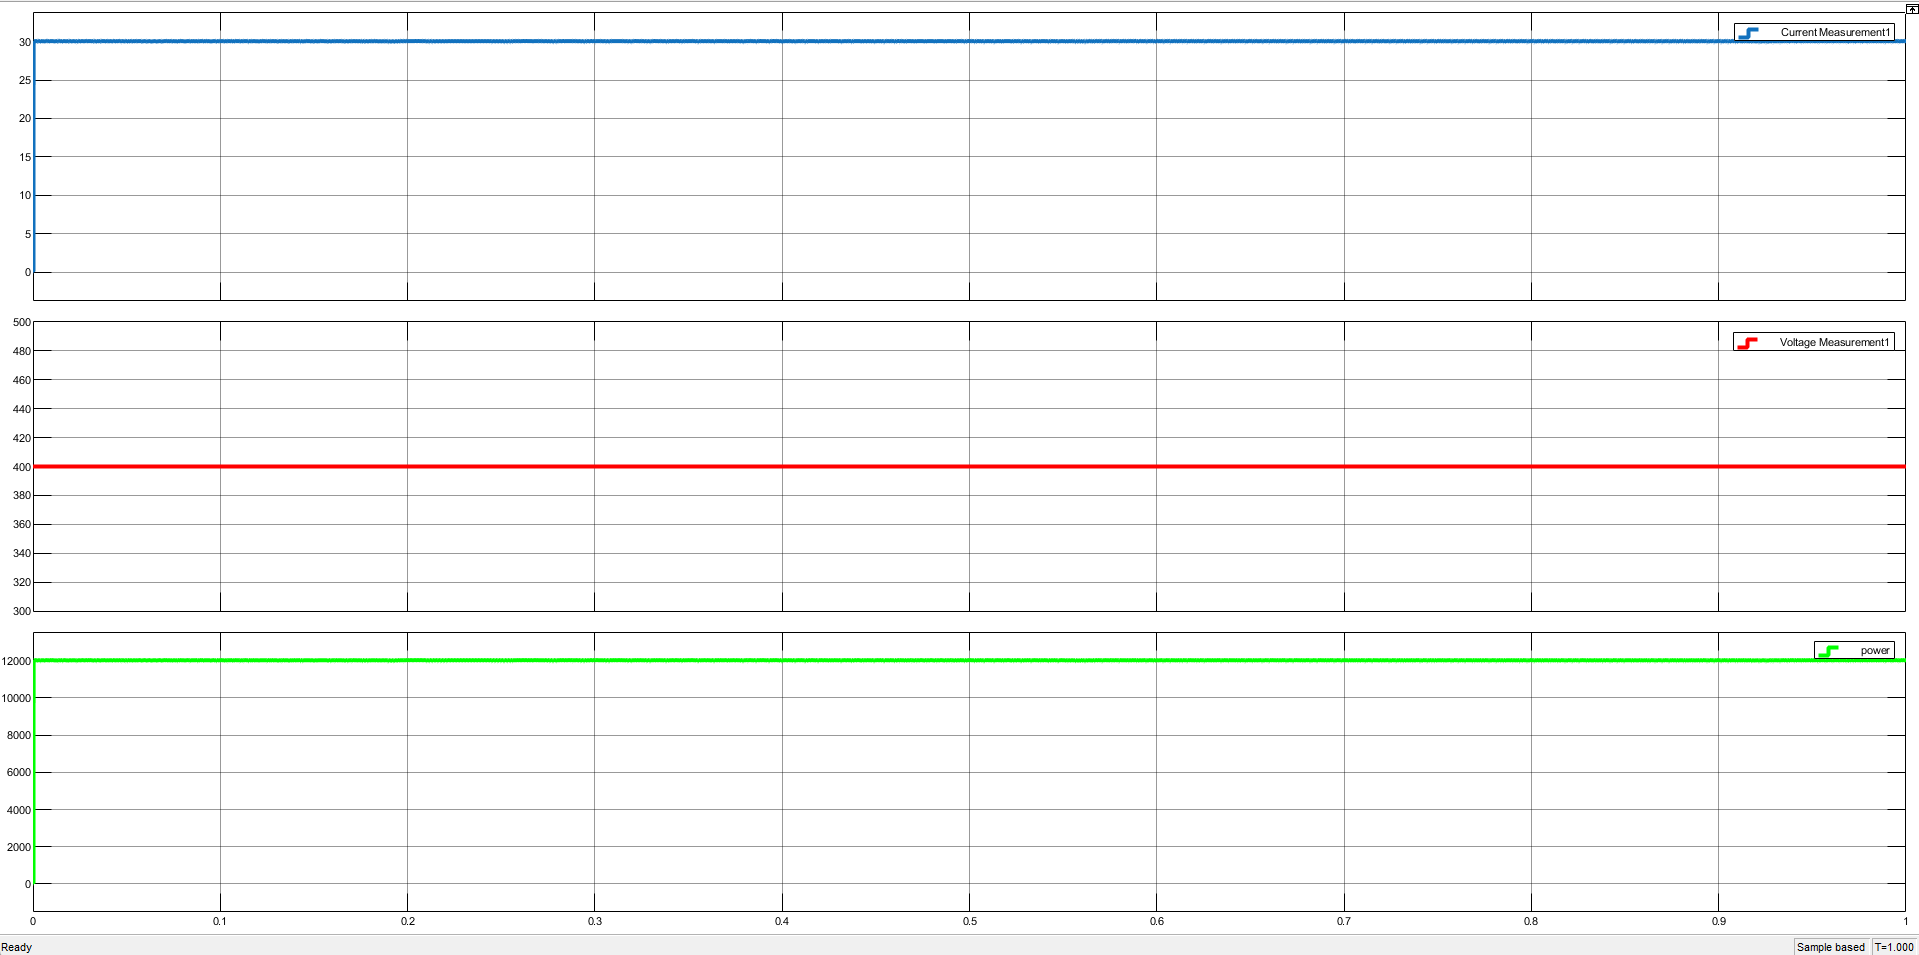
\includegraphics[width=1\textwidth]{Figures/5.4.18.png}
    \caption{Ibattery, Vbattery, Pbattery.}
    \label{Ibattery , Vbattery , Pbattery of all system2}
\end{figure}

\begin{figure}[H]
    \centering
    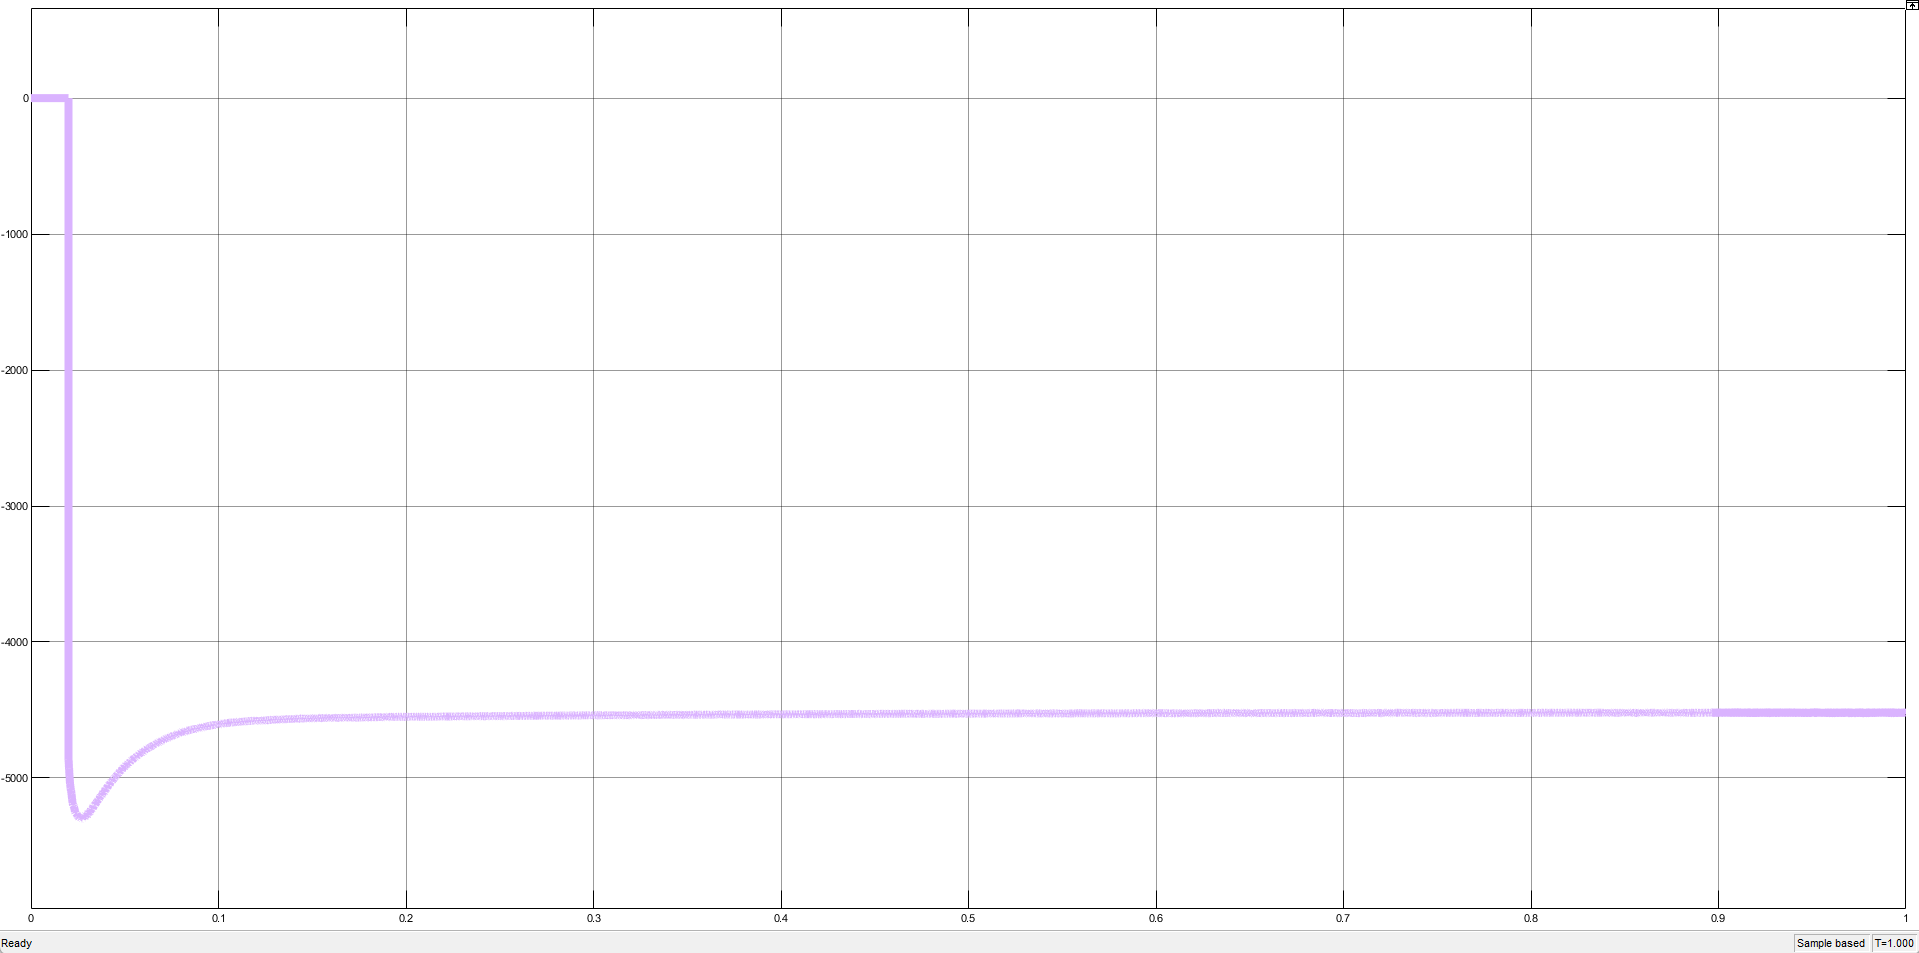
\includegraphics[width=1\textwidth]{Figures/5.4.19.png}
    \caption{Grid Power.}
    \label{grid power of the system2}
\end{figure}

\subsection{Simulation of the Off-Grid System (High Ratings)}

\subsubsection{System Modeling and Converter Design}

\begin{figure}[H]
    \centering
    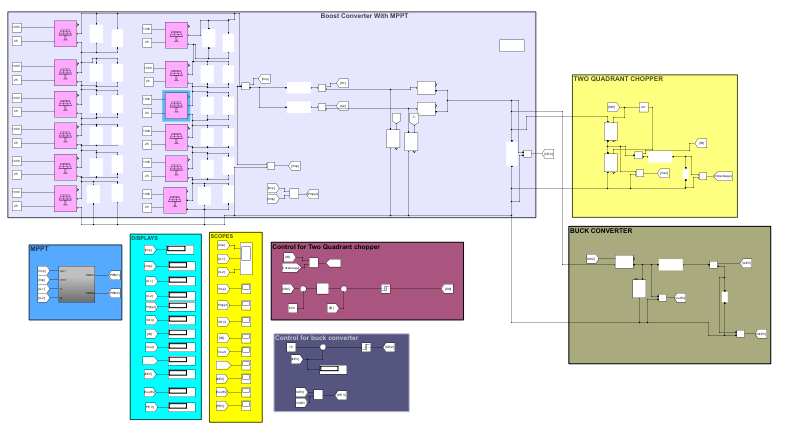
\includegraphics[width=0.9\textwidth]{Figures/full.png}
    \caption{Full System}
    \label{fig:full_system}
\end{figure}

\paragraph{PV Array Specifications}

The photovoltaic (PV) system serves as the primary power source for the overall system. The PV array is designed using a centralized topology to minimize complexity and cost. It consists of six individual PV modules connected in series to form a single string, while two strings are connected in parallel. Based on the specifications of a single PV module, the overall array characteristics under Standard Test Conditions (STC: 1000~W/m$^{2}$, 25$^\circ$C) are calculated as follows.

\begin{align}
V_{MPP} &= 6 \times 40.9 = 245.4~\text{V}
\end{align}

\begin{align}
I_{MPP} &= 2 \times 17.36 = 34.72~\text{A}
\end{align}

\begin{align}
V_{OC} &= 294~\text{V}
\end{align}

\begin{align}
I_{SC} &= 2 \times 18.4 = 36.8~\text{A}
\end{align}

\begin{align}
P_{MAX} &= 245.4 \times 34.72 = 8520~\text{W}
\end{align}

\begin{table}[H]
\centering
\caption{PV Array Specifications}
\label{tab:pv_specifications}
\begin{tabular}{|l|c|}
\hline
\textbf{Parameter} & \textbf{Value} \\
\hline
Voltage at Maximum Power ($V_{MPP}$) & 245.4 V \\
Current at Maximum Power ($I_{MPP}$) & 34.72 A \\
Open-Circuit Voltage ($V_{OC}$) & 294 V \\
Short-Circuit Current ($I_{SC}$) & 36.8 A \\
Maximum Output Power ($P_{MAX}$) & 8520 W \\
\hline
\end{tabular}
\end{table}

\begin{figure}[H]
    \centering
    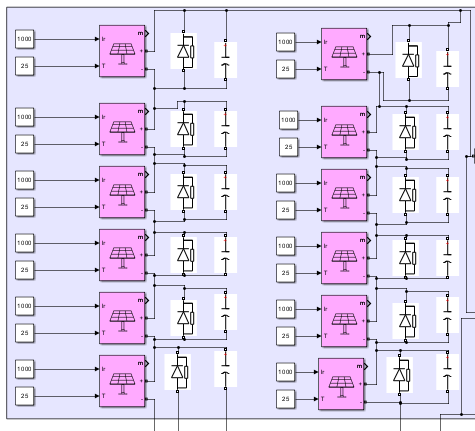
\includegraphics[width=0.8\textwidth]{Figures/pvm.png}
    \caption{PV Modules}
    \label{fig:mpp_current}
\end{figure}
\begin{figure}[H]
    \centering
    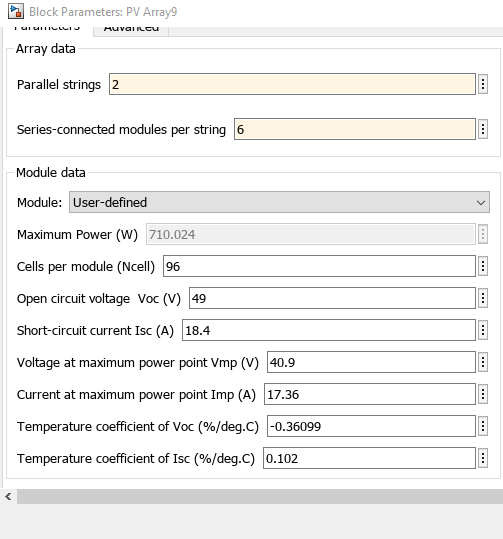
\includegraphics[width=0.8\textwidth]{Figures/rating.png}
    \caption{Rating of One Module}
    \label{fig:mpp_current}
\end{figure}
\begin{figure}[H]
    \centering
    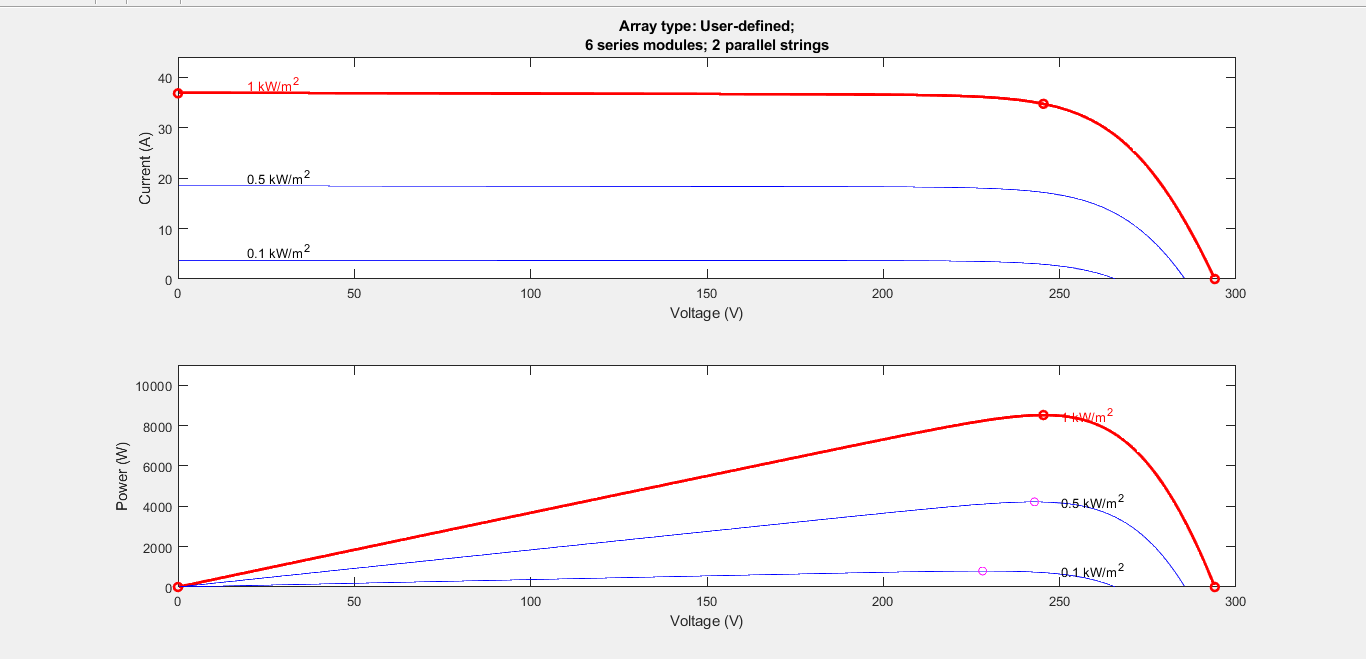
\includegraphics[width=0.8\textwidth]{Figures/mppt2.png}
    \caption{Max Power point }
    \label{fig:mpp_current}
\end{figure}

\subsubsection{Boost Converter and MPPT Operation}

\begin{figure}[H]
    \centering
    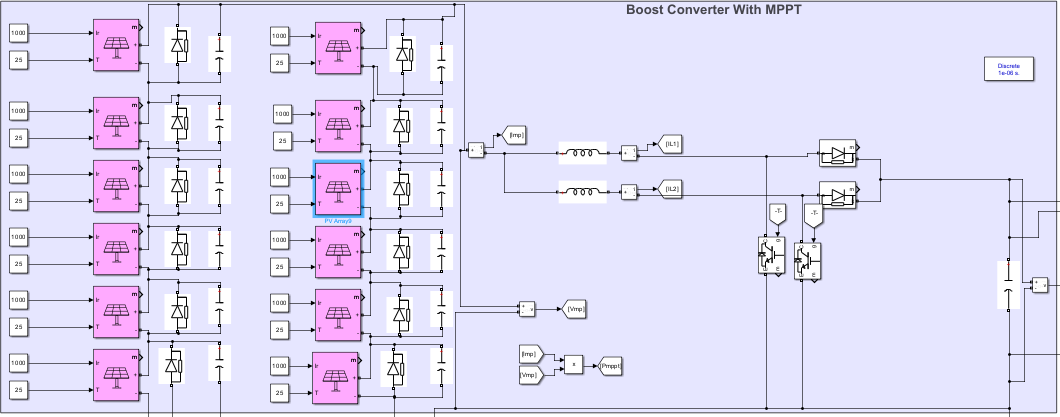
\includegraphics[width=0.8\textwidth]{Figures/boost.png}
    \caption{Boost Converter}
    \label{fig:boost_converter}
\end{figure}

Since the output voltage of the PV array ($245.4~\mathrm{V}$) fluctuates continuously due to variations in solar irradiance and temperature, and is typically lower than the required common DC bus voltage, a DC--DC Boost Converter is integrated. This converter performs two critical functions.

\paragraph{Voltage Stepping-Up}

The converter regulates and steps up the fluctuating PV array voltage to maintain a stable DC bus voltage of $600~\mathrm{V}$. Based on the continuous conduction mode (CCM) equation of the boost converter, the theoretical duty cycle at the maximum power point is calculated as follows:

\begin{equation}
D = 1-\frac{V_{in}}{V_{out}}
\end{equation}

\begin{equation}
D = 1-\frac{245.4}{600}=0.591
\end{equation}

This indicates that the converter operates with a nominal duty cycle of approximately $59.1\%$ under Standard Test Conditions (STC).

\paragraph{Maximum Power Extraction}

The duty cycle of the boost converter is controlled by a Maximum Power Point Tracking (MPPT) algorithm. This ensures that the PV array continuously operates at its optimal voltage and current, extracting the maximum available electrical power of approximately $8520~\mathrm{W}$ despite environmental variations.
\newpage
\subsubsection{Internal Architecture of the MPPT Subsystem}

This subsystem is implemented based on the Perturb and Observe (P\&O) algorithm [5]. The operational mechanism consists of the following stages:

\begin{itemize}

\item \textbf{Power Change ($\Delta P$) Calculation}

The instantaneous PV voltage ($V_{pv1}$) and current ($I_{pv1}$) are measured and multiplied to calculate the output power

\begin{equation}
P=V\times I
\end{equation}

The previous power value is stored using a Unit Delay ($1/z$) block and compared with the current value to calculate the power variation ($\Delta P$).

\item \textbf{Reference Current Generation}

According to the sign of $\Delta P$, the controller increments or decrements the reference current ($I_{ref}$) using a fixed step size of $0.05$. This iterative process continuously drives the operating point toward the maximum power point.

\item \textbf{Dual PI Current Control}

Since an Interleaved Boost Converter is employed, the generated reference current is divided between the two converter phases and compared with the measured inductor currents ($I_1$ and $I_2$). Two independent PI controllers regulate each phase to minimize the steady-state current error.

\item \textbf{Interleaved PWM Signal Generation}

Two PWM signals ($PWM_1$ and $PWM_2$) are generated with an accurate $180^\circ$ phase shift using a Delay block. This interleaving technique ensures balanced current sharing between the converter phases, significantly reducing the input current ripple and decreasing the electrical stress on the switching devices.

\end{itemize}

\begin{figure}[H]
    \centering
    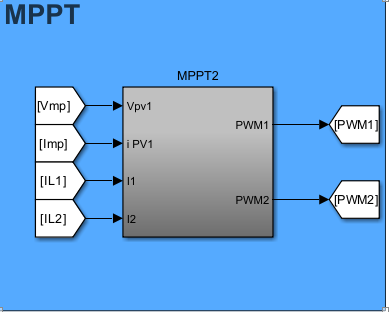
\includegraphics[width=0.8\textwidth]{Figures/mppt block.png}
    \caption{MPPT block}
    \label{fig:mppt_architecture}
\end{figure}
\begin{figure}[H]
    \centering
    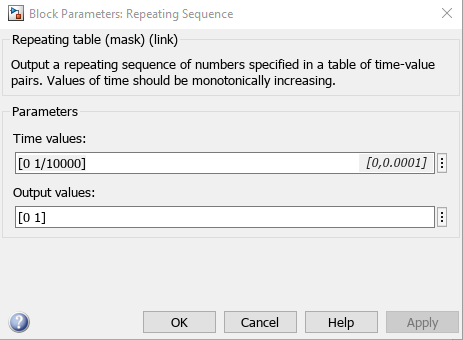
\includegraphics[width=0.8\textwidth]{Figures/repeating sequence.png}
    \caption{Repeating sequence}
    \label{fig:mppt_architecture}
\end{figure}
\begin{figure}[H]
    \centering
    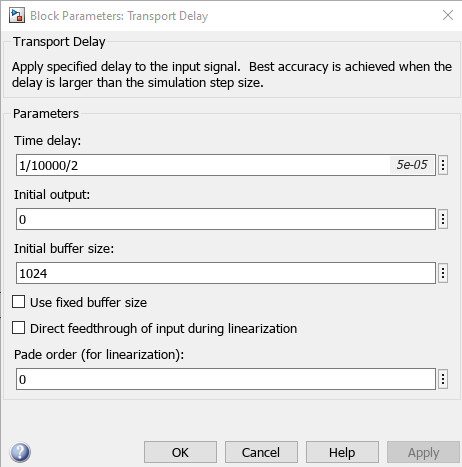
\includegraphics[width=0.8\textwidth]{Figures/transport delay.png}
    \caption{Transport Delay}
    \label{fig:mppt_architecture}
\end{figure}
\begin{figure}[H]
    \centering
    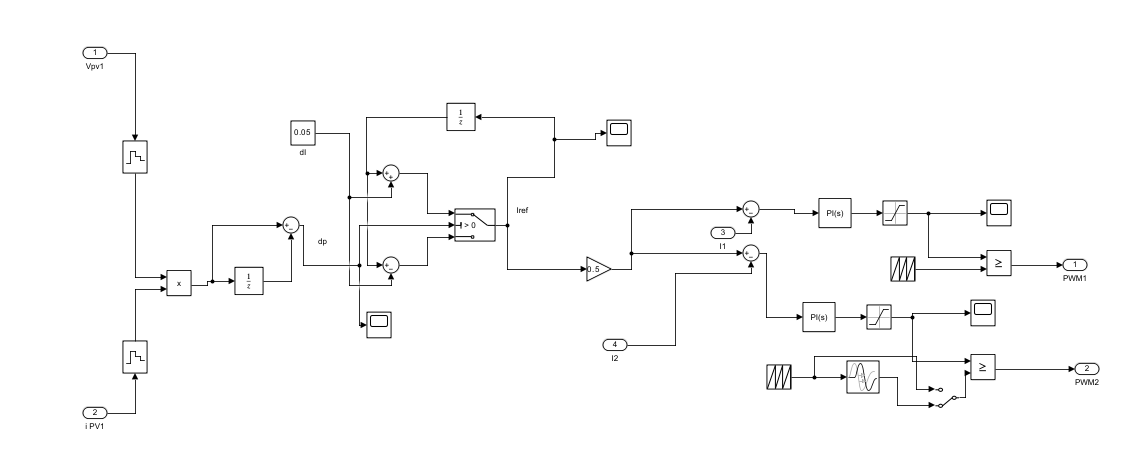
\includegraphics[width=0.8\textwidth]{Figures/intrenal struvture.png}
    \caption{Internal Architecture of the MPPT }
    \label{fig:mppt_architecture}
\end{figure}

\subsubsection{MPPT Using MATLAB Function Block}

To improve power extraction efficiency and reduce the effects of partial shading, a Global Maximum Power Point Tracking (GMPPT) algorithm was implemented using a MATLAB Function block. The algorithm is based on a voltage sweep technique consisting of an outer voltage loop and an inner current control loop.

\paragraph{Voltage Sweep Logic}

The algorithm operates through a finite-state machine with four operating modes:

\begin{itemize}
    \item RESET
    \item SCAN
    \item RETURN
    \item HOLD
\end{itemize}

Initially, the RESET mode drives the PV voltage toward the estimated open-circuit voltage ($250~\mathrm{V}$). During the SCAN mode, the reference voltage is gradually decreased while monitoring the generated power. The algorithm records the global maximum power ($P_{max}$) together with its corresponding voltage ($V_{best}$). The RETURN mode then smoothly drives the operating point back to $V_{best}$, while the HOLD mode maintains this operating point for five seconds before initiating a new sweep cycle.

\paragraph{Inner Current Control Loop}

To force the PV array to accurately track the desired target voltage ($V_{target}$), a digital PI controller with an anti-windup mechanism is implemented. The controller continuously calculates the voltage error and updates the reference current ($I_{ref}$). For safe converter operation, the reference current is limited within the range

\[
0 \le I_{ref} \le 35~\mathrm{A}
\]

which guarantees stable and reliable boost converter performance.

\begin{figure}[H]
    \centering

    \begin{subfigure}[t]{0.4\textwidth}
        \centering
        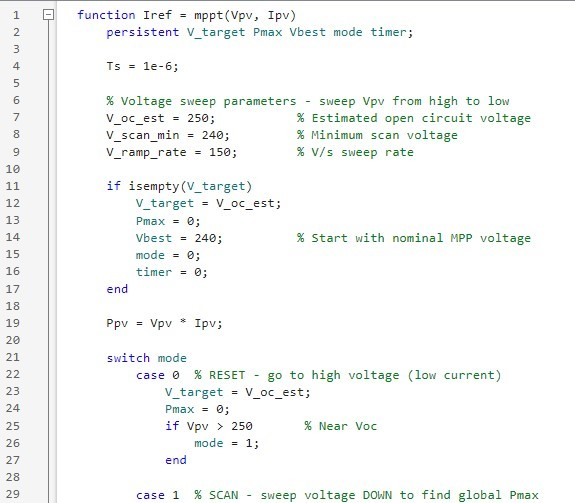
\includegraphics[width=\linewidth]{Figures/mppt1.jpg}
    \end{subfigure}
    \hfill
    \begin{subfigure}[t]{0.4\textwidth}
        \centering
        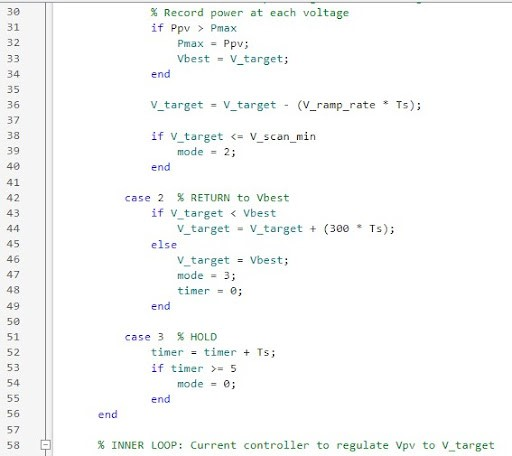
\includegraphics[width=\linewidth]{Figures/mppt2.jpg}
    \end{subfigure}
    \hfill
    \begin{subfigure}[t]{0.4\textwidth}
        \centering
        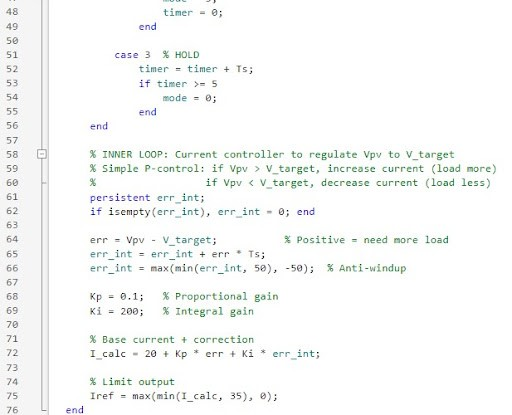
\includegraphics[width=\linewidth]{Figures/mppt3.jpg}
    \end{subfigure}

    \caption{MATLAB implementation of the Global Maximum Power Point Tracking (GMPPT) algorithm using the voltage sweep technique.}
    \label{fig:gmppt_code}
\end{figure}

\subsubsection{Two-Quadrant Chopper}

\paragraph{Primary Function and Operation Modes}

The primary purpose of this circuit is to manage the power flow between the common DC bus and the energy storage system (battery). The converter allows bidirectional power transfer, enabling battery charging from the DC bus in \textbf{Buck mode} and battery discharging to the DC bus in \textbf{Boost mode}.

\begin{figure}[H]
    \centering
    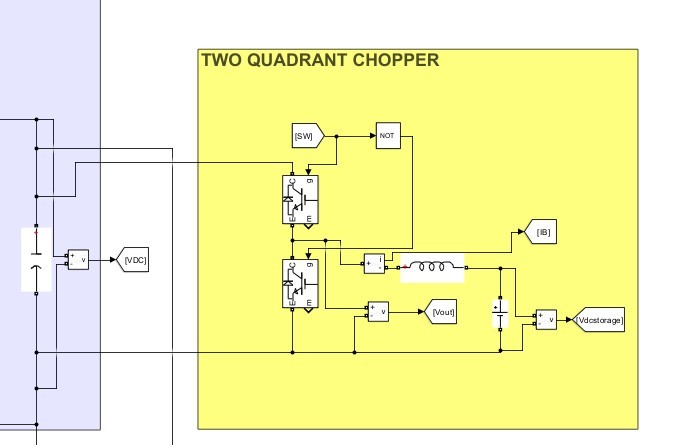
\includegraphics[width=0.7\textwidth]{Figures/2q.jpg}
    \caption{Two-Quadrant Chopper}
    \label{fig:two_quadrant}
\end{figure}

\paragraph{Control Strategy}

The converter employs a closed-loop current control strategy to ensure accurate charging and discharging of the battery. The actual battery current is continuously measured and compared with the reference current. The resulting error is processed by the controller to generate the switching signal.

The generated PWM signal is applied directly to the gate of the first switch, while the complementary signal is obtained through a logical \textbf{NOT} gate and applied to the second switch. This complementary switching guarantees safe converter operation and prevents a short circuit across the DC bus.

\begin{figure}[H]
    \centering
    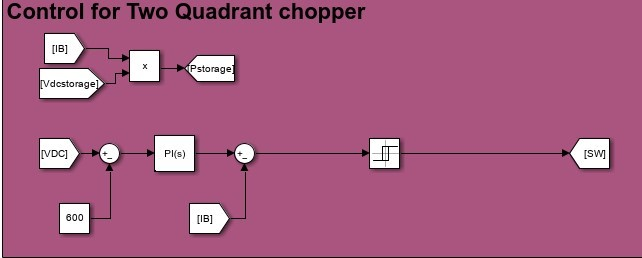
\includegraphics[width=0.7\textwidth]{Figures/2q control.jpg}
    \caption{Control of the Two-Quadrant Chopper}
    \label{fig:two_quadrant_control}
\end{figure}

%%%%%%%%%%%%%%%%%%%%%%%%%%%%%%%%%%%%%%%%%%%%%%%%%%%%%%%%%%%

\subsubsection{DC Buck Converter}

\paragraph{Primary Function}

The DC Buck Converter serves as the final power stage of the system. Its primary function is to step down the common DC bus voltage to a lower regulated voltage suitable for charging the Electric Vehicle (EV) battery. The converter delivers a constant charging current to ensure safe and reliable battery charging.

\begin{figure}[H]
    \centering
    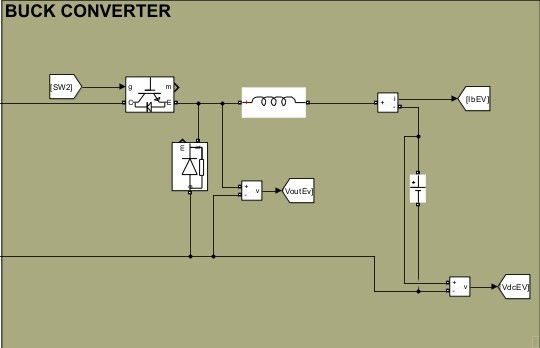
\includegraphics[width=0.8\textwidth]{Figures/buck.jpg}
    \caption{DC Buck Converter}
    \label{fig:buck_converter}
\end{figure}

\paragraph{Control Strategy}

The buck converter employs a closed-loop control system based on the Hysteresis Current Control technique, which is characterized by its fast dynamic response and high current regulation accuracy.

The control strategy consists of the following stages:

\begin{itemize}
    \item \textbf{Current Loop:} A constant reference current of $10~\mathrm{A}$ is defined and continuously compared with the measured EV battery current ($I_{bEV}$).

    \item \textbf{Pulse Generation:} The current error is applied to a Relay block acting as a hysteresis controller. The Relay generates the switching pulses ($SW_2$), forcing the output current to remain within a narrow hysteresis band around the 10 A reference.

    \item \textbf{Power Calculation:} An additional subsystem calculates the instantaneous EV charging power ($P_{EV}$) by multiplying the measured output voltage ($V_{dcEV}$) by the measured battery current ($I_{bEV}$):

    \begin{equation}
    P_{EV}=V_{dcEV}\times I_{bEV}
    \end{equation}

    \begin{figure}[H]
    \centering
    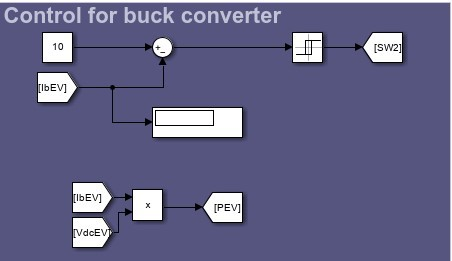
\includegraphics[width=0.8\textwidth]{Figures/buckcontrol.jpg}
    \caption{Converter for buck converter}
    \label{fig:buck_converter}
\end{figure}

\subsection{Results}

\subsubsection{Case 1}

The simulation validates the system's ability to manage power distribution dynamically. Under the defined operating scenario, the PV source successfully supplies power to both the EV load and the energy storage system (ESS). The obtained simulation results are summarized in Table~\ref{tab:case1}.

\begin{table}[H]
\centering
\caption{Simulation Results for Case 1}
\label{tab:case1}
\begin{tabular}{|l|c|}
\hline
\textbf{Parameter} & \textbf{Value} \\
\hline
DC Link Voltage & 600 V \\
EV Reference Current & 10 A \\
EV Battery Voltage & 400 V \\
Storage Battery Voltage & 400 V \\
PV Voltage at MPP & 245.4 V \\
PV Current at MPP & 34.7 A \\
PV Maximum Power & 8520 W \\
EV Battery Power & 4000 W \\
Storage Battery Power & 4520 W \\
Two-Quadrant Chopper Mode & Buck (Charging) \\
\hline
\end{tabular}
\end{table}

\paragraph{Performance Evaluation}

\begin{itemize}

\item \textbf{Load Regulation:}
The hysteresis current controller successfully regulates the EV charging current at 10 A, providing a constant charging power of approximately 4000 W despite variations in the DC bus voltage.

\item \textbf{ESS Management:}
The bidirectional converter operates in Buck mode to charge the energy storage system using the surplus PV power (4520 W). The simulation confirms efficient power transfer and accurate charging current regulation.

\item \textbf{System Stability:}
The obtained waveforms demonstrate fast transient response and stable operation of the DC bus voltage while simultaneously supplying the EV load and charging the ESS, validating the effectiveness of the overall control strategy.

\end{itemize}

\paragraph{Scopes and Displays}


%%%%%%%%%%%%%%%%%%%%%%%%%%%%%%%%%%%%%%%%%%%%%%%%%%%%%%%
\begin{figure}[H]
\centering
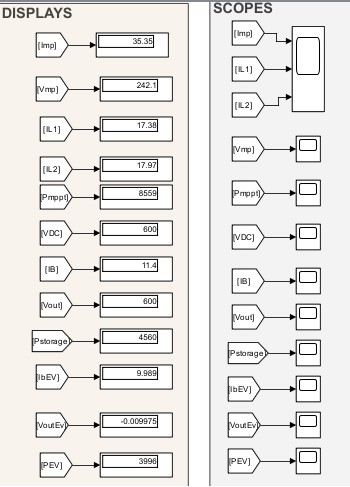
\includegraphics[width=0.8\textwidth]{Figures/yarab.jpg}
\caption{Scopes and Displays}
\label{fig:interleaved_current}
\end{figure}

\begin{figure}[H]
\centering
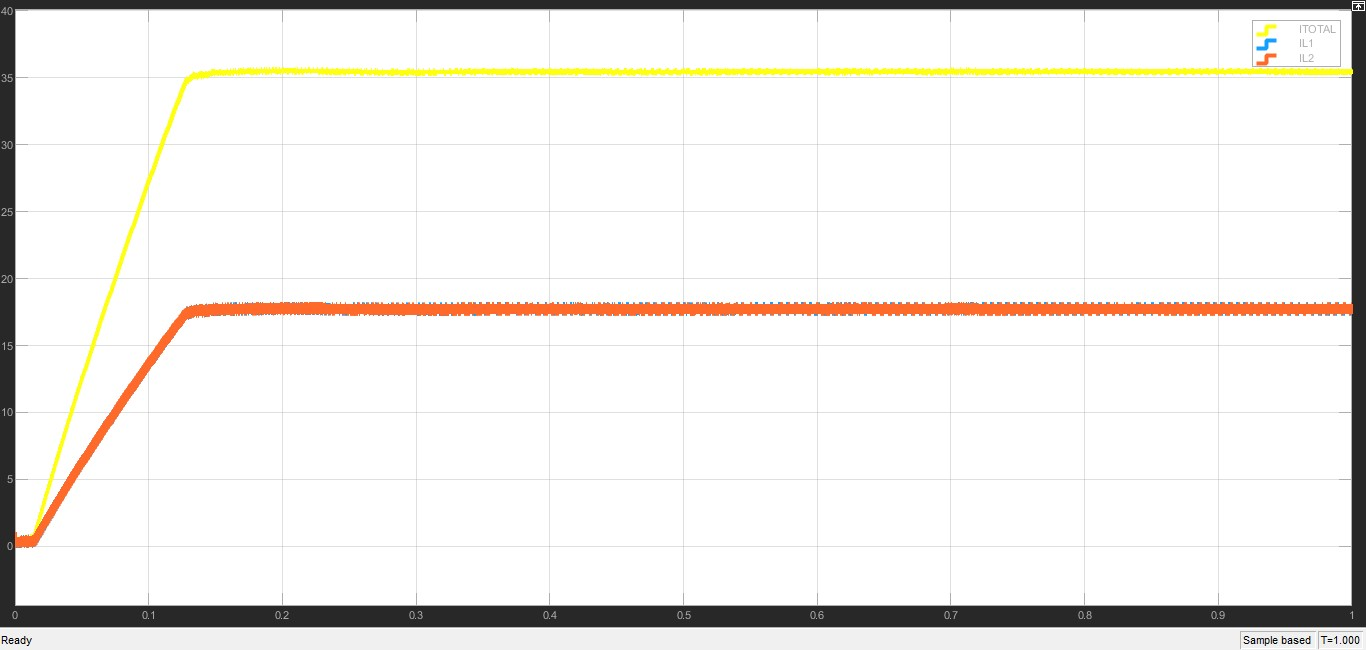
\includegraphics[width=0.8\textwidth]{Figures/Inew.jpg}
\caption{Total Input Current versus Inductor Currents ($I_{L1}$ and $I_{L2}$)}
\label{fig:interleaved_current}
\end{figure}

\begin{figure}[H]
\centering
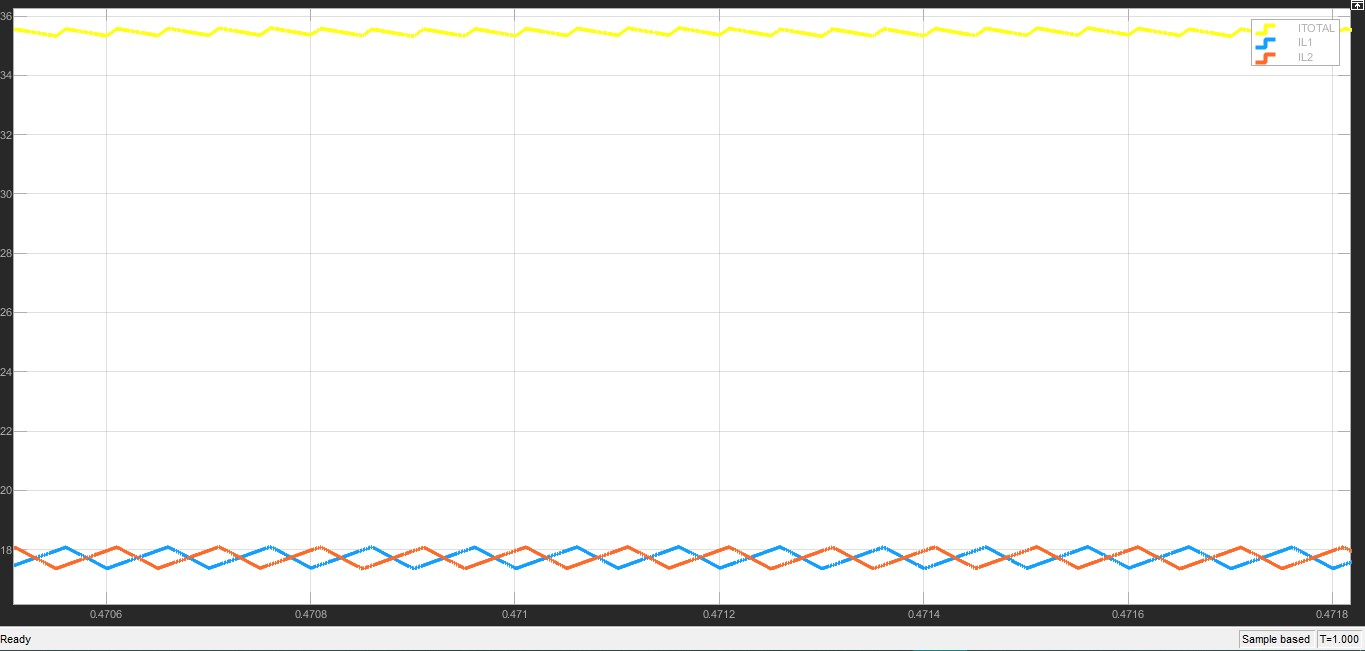
\includegraphics[width=0.8\textwidth]{Figures/I2.jpg}
\caption{ Zoom in for Total Input Current versus Inductor Currents ($I_{L1}$ and $I_{L2}$)}
\label{fig:interleaved_current}
\end{figure}
The waveform demonstrates the effectiveness of the 180$^\circ$ interleaving technique. The ripple components of the individual inductor currents cancel each other, resulting in a smoother total input current compared with a conventional single-phase boost converter.

%%%%%%%%%%%%%%%%%%%%%%%%%%%%%%%%%%%%%%%%%%%%%%%%%%%%%%%

\begin{figure}[H]
\centering
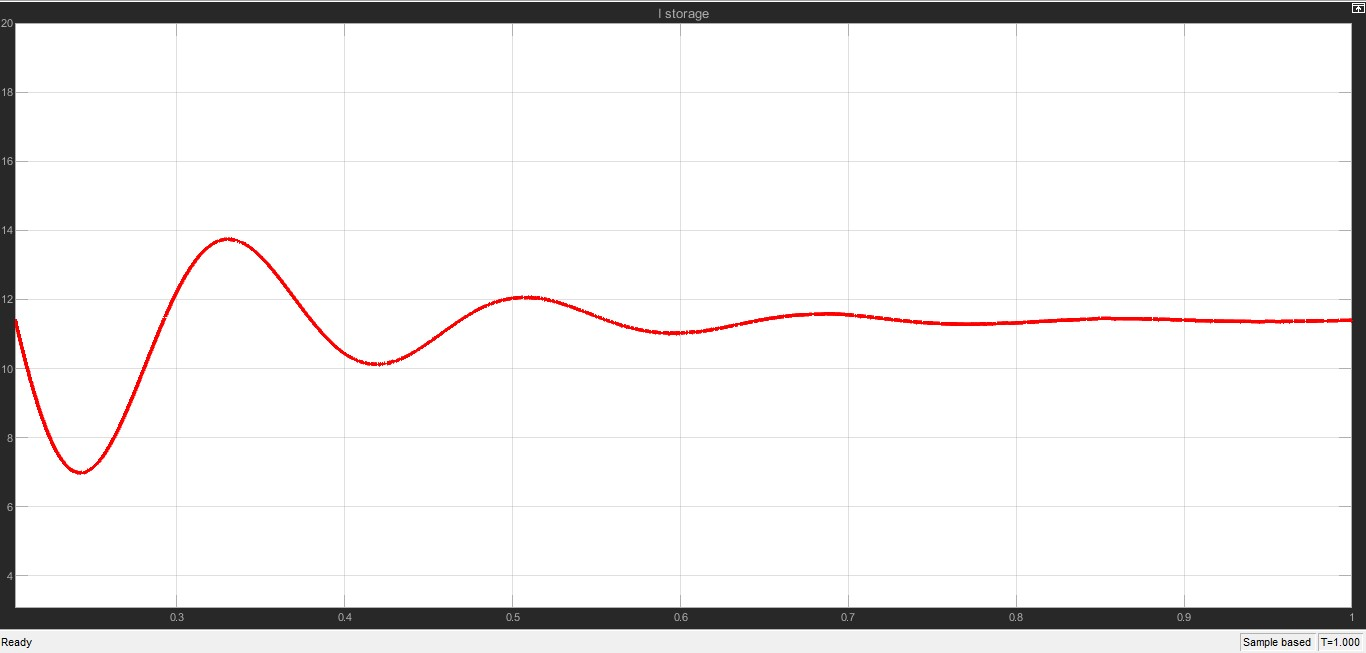
\includegraphics[width=\textwidth]{Figures/IBattery storage.jpg}
\caption{Energy Storage System (ESS) Charging Current}
\label{fig:ess_current}
\end{figure}

The waveform illustrates the transient charging response followed by a stable steady-state current, confirming the effectiveness of the PI current controller.

%%%%%%%%%%%%%%%%%%%%%%%%%%%%%%%%%%%%%%%%%%%%%%%%%%%%%%%

\begin{figure}[H]
\centering
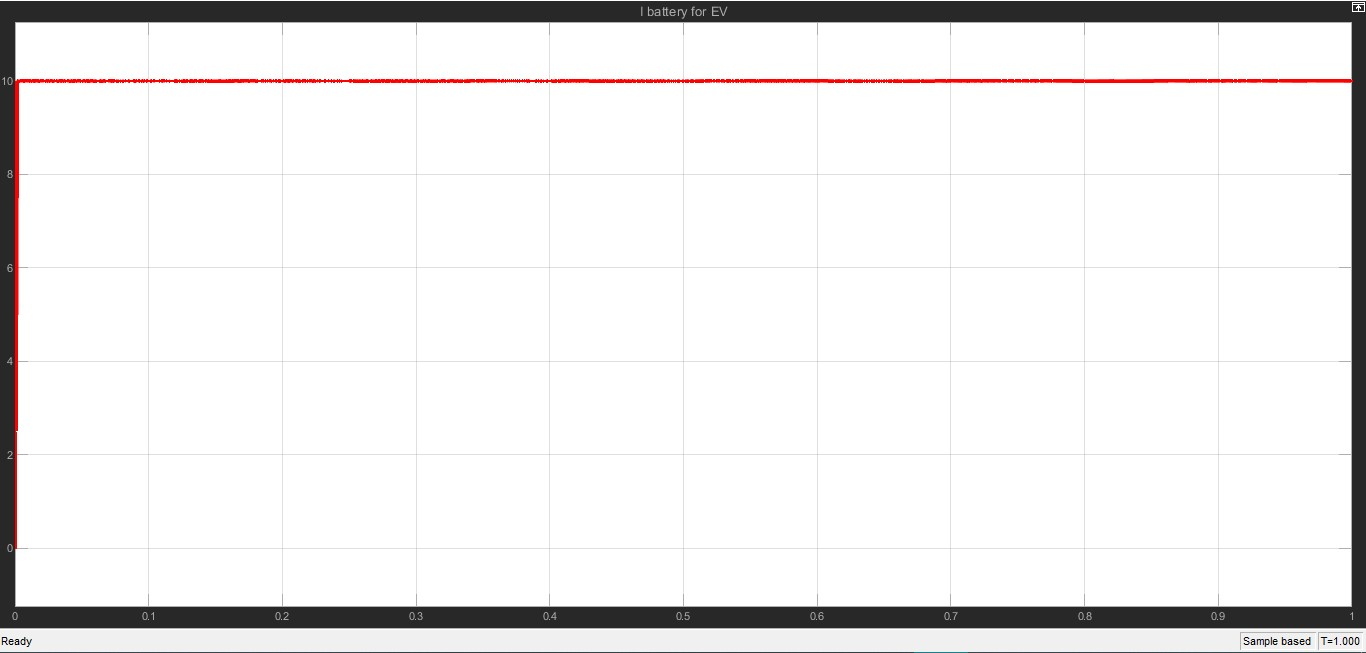
\includegraphics[width=0.8\textwidth]{Figures/iev.jpg}
\caption{EV Battery Charging Current}
\label{fig:ev_current}
\end{figure}

The hysteresis current controller maintains the EV charging current at the desired reference value of 10 A with excellent regulation accuracy.

%%%%%%%%%%%%%%%%%%%%%%%%%%%%%%%%%%%%%%%%%%%%%%%%%%%%%%%

\begin{figure}[H]
\centering
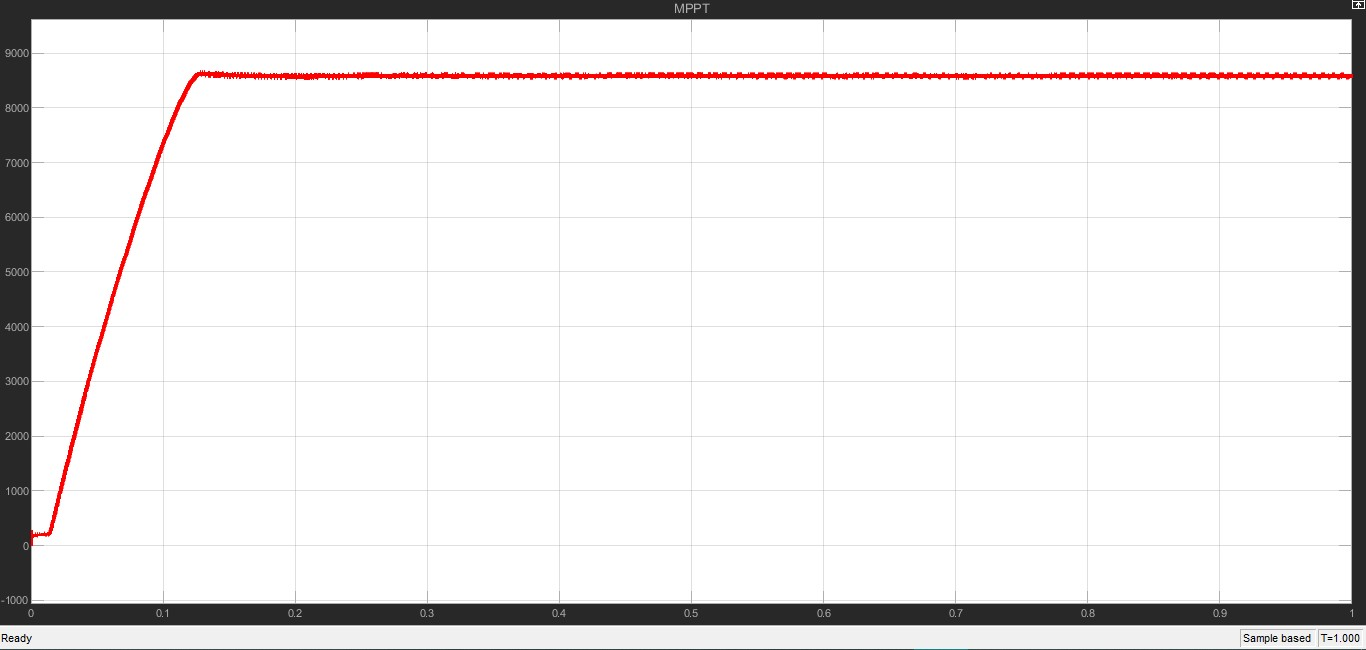
\includegraphics[width=0.8\textwidth]{Figures/pmppt.jpg}
\caption{PV Array Power Tracked by the MPPT Algorithm}
\label{fig:mppt_power}
\end{figure}

The MPPT algorithm rapidly converges to the maximum available power of approximately 8.52 kW and maintains stable operation around the maximum power point.

%%%%%%%%%%%%%%%%%%%%%%%%%%%%%%%%%%%%%%%%%%%%%%%%%%%%%%%

\begin{figure}[H]
\centering
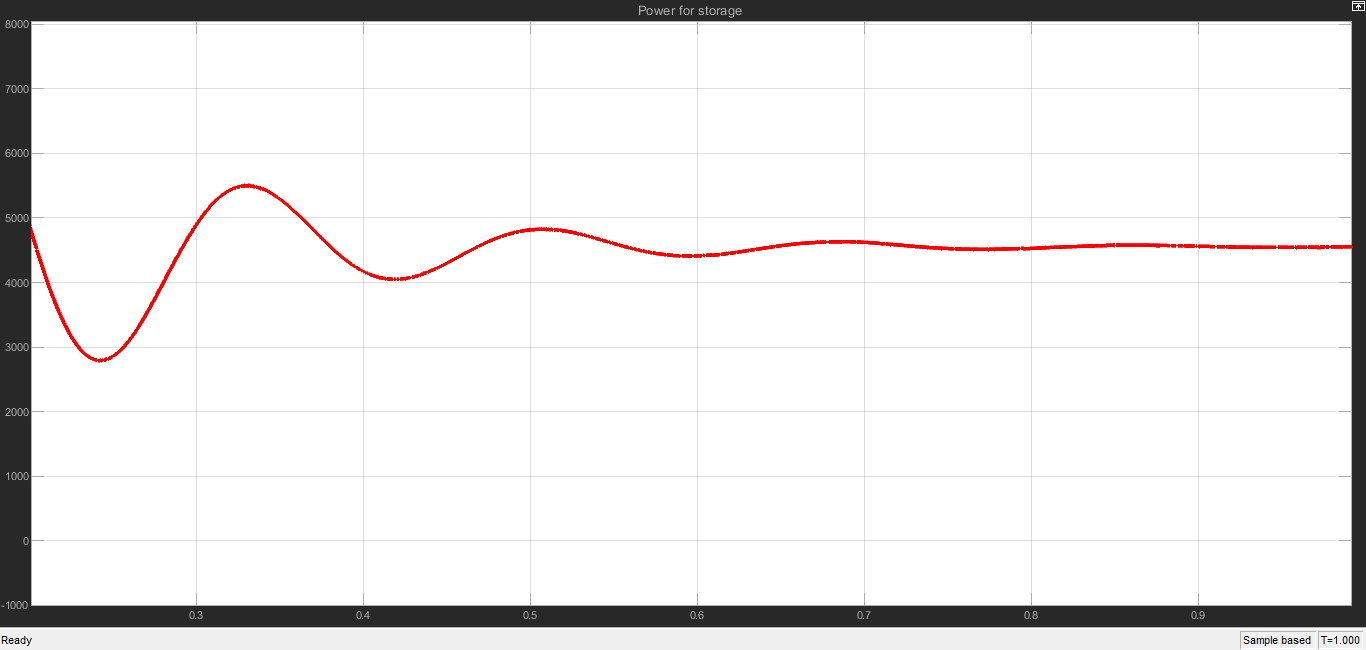
\includegraphics[width=0.8\textwidth]{Figures/pout for storage.jpg}
\caption{Storage Battery Power}
\label{fig:storage_power}
\end{figure}

The waveform confirms that approximately 4.52 kW of surplus power is efficiently transferred to the ESS during the charging process.

%%%%%%%%%%%%%%%%%%%%%%%%%%%%%%%%%%%%%%%%%%%%%%%%%%%%%%%

\begin{figure}[H]
\centering
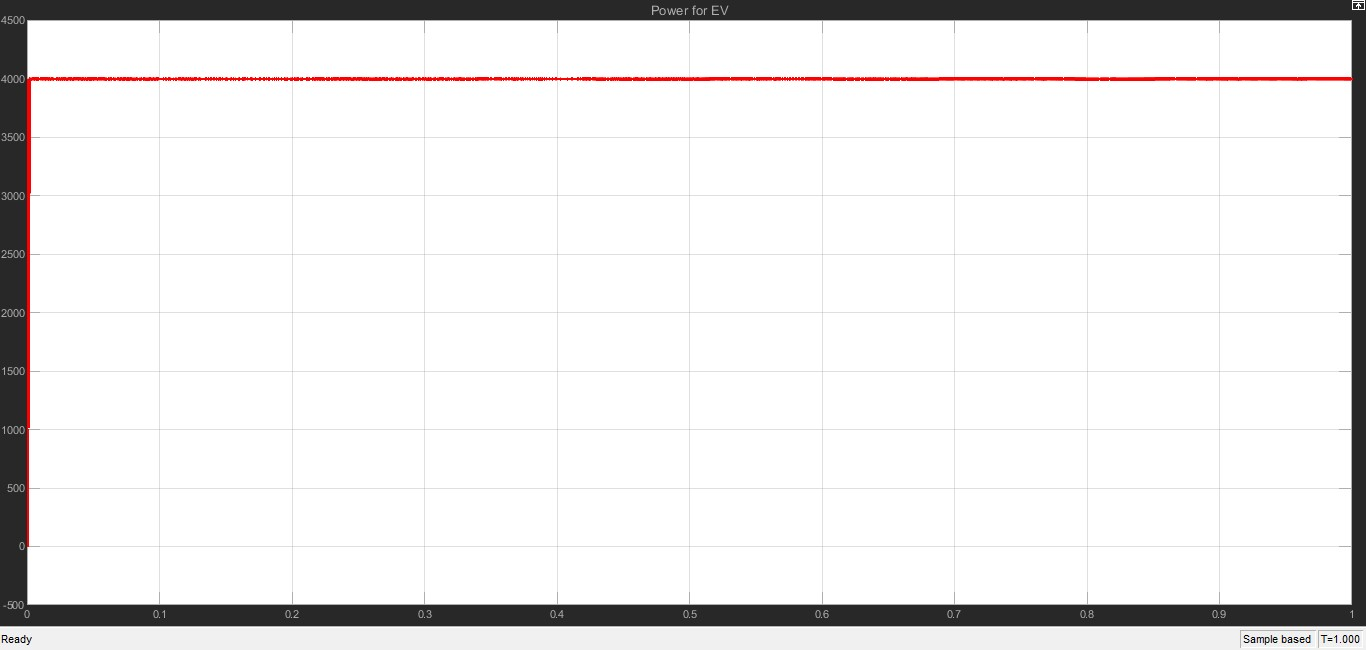
\includegraphics[width=0.8\textwidth]{Figures/Powerev.jpg}
\caption{EV Load Power}
\label{fig:ev_power}
\end{figure}

The EV charging power remains constant at approximately 4 kW, indicating stable operation throughout the charging interval.

%%%%%%%%%%%%%%%%%%%%%%%%%%%%%%%%%%%%%%%%%%%%%%%%%%%%%%%

\begin{figure}[H]
\centering
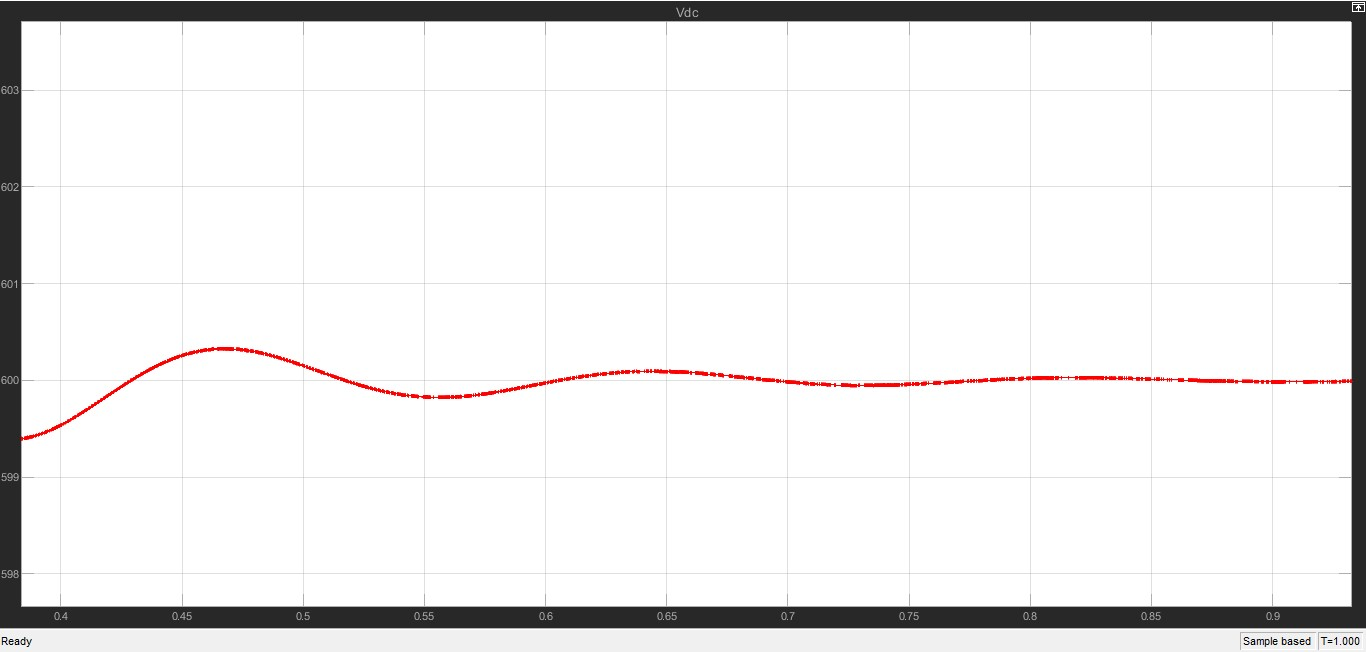
\includegraphics[width=0.8\textwidth]{Figures/vdc.jpg}
\caption{DC Bus Voltage}
\label{fig:dc_bus}
\end{figure}

The DC bus voltage is successfully regulated at 600 V with minimal ripple, demonstrating the effectiveness of the integrated control strategy.

%%%%%%%%%%%%%%%%%%%%%%%%%%%%%%%%%%%%%%%%%%%%%%%%%%%%%%%

\begin{figure}[H]
\centering
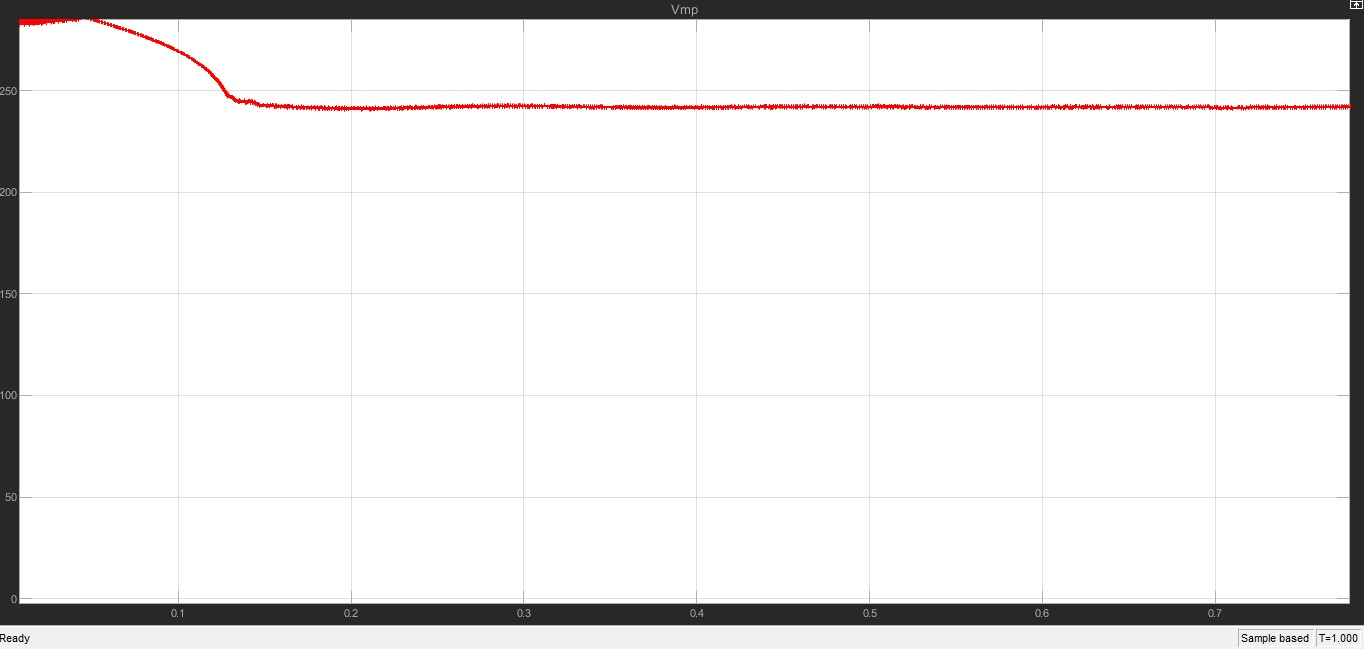
\includegraphics[width=0.8\textwidth]{Figures/vmp.jpg}
\caption{PV Array Voltage at the Maximum Power Point}
\label{fig:pv_voltage}
\end{figure}

The PV voltage remains close to the desired maximum power point voltage (245.4 V), indicating high MPPT tracking accuracy and stable converter operation.

\subsubsection{Case 2}

The simulation validates the system's ability to maintain power balance under deficit conditions, where the EV load demand exceeds the available PV generation. The system performance is summarized in Table~\ref{tab:case2}.

\begin{table}[H]
\centering
\caption{Simulation Results for Case 2}
\label{tab:case2}
\begin{tabular}{|l|c|}
\hline
\textbf{Parameter} & \textbf{Value} \\
\hline
PV Generated Power & 8520 W \\
EV Load Power & 12000 W \\
ESS Compensation Power & 3480 W (Discharging) \\
Two-Quadrant Chopper Mode & Boost (Discharging) \\
\hline
\end{tabular}
\end{table}

\paragraph{Performance Evaluation}

\begin{itemize}

\item \textbf{Power Balancing Logic:}

The simulation demonstrates that the system successfully maintains instantaneous power balance by supplying the required deficit power from the Energy Storage System (ESS). The required compensation power is

\begin{equation}
P_{ESS}=12000-8520=3480~\mathrm{W}
\end{equation}

which enables the EV load demand to be fully satisfied.

\item \textbf{Bidirectional Converter Operation:}

During this operating condition, the Two-Quadrant Chopper automatically switches to the \textbf{Boost} operating mode. The battery discharge current confirms that energy is transferred from the ESS to the DC bus while maintaining the DC bus voltage at 600 V.

\item \textbf{System Stability:}

Although the EV load requires 12 kW, the integrated control strategy successfully regulates the DC bus voltage at 600 V, demonstrating the robustness of the proposed system during power deficit conditions.

\end{itemize}

\paragraph{Scopes and Displays}

%%%%%%%%%%%%%%%%%%%%%%%%%%%%%%%%%%%%%%%%%%%%%%%%%%%%%%%%%%

\begin{figure}[H]
\centering
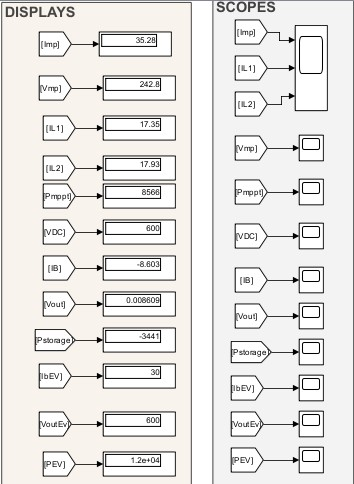
\includegraphics[width=0.9\textwidth]{Figures/SharedScreenshot.jpg}
\caption{Scopes and Displays}
\label{fig:case2_scope}
\end{figure}

%%%%%%%%%%%%%%%%%%%%%%%%%%%%%%%%%%%%%%%%%%%%%%%%%%%%%%%%%%

\begin{figure}[H]
\centering
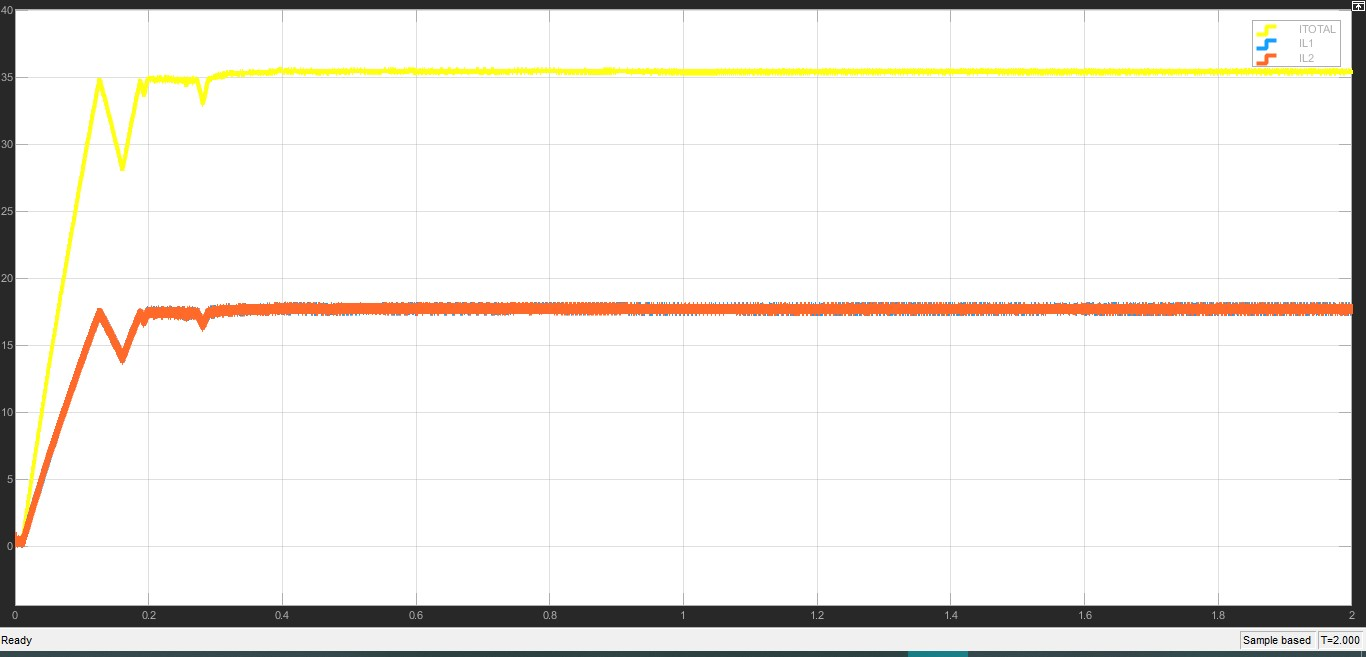
\includegraphics[width=0.85\textwidth]{Figures/case2/inew.jpg}
\caption{Interleaved Inductor Currents ($I_{L1}$ and $I_{L2}$) and Total Input Current During Boost Mode}
\label{fig:interleaved_case2}
\end{figure}

\begin{figure}[H]
\centering
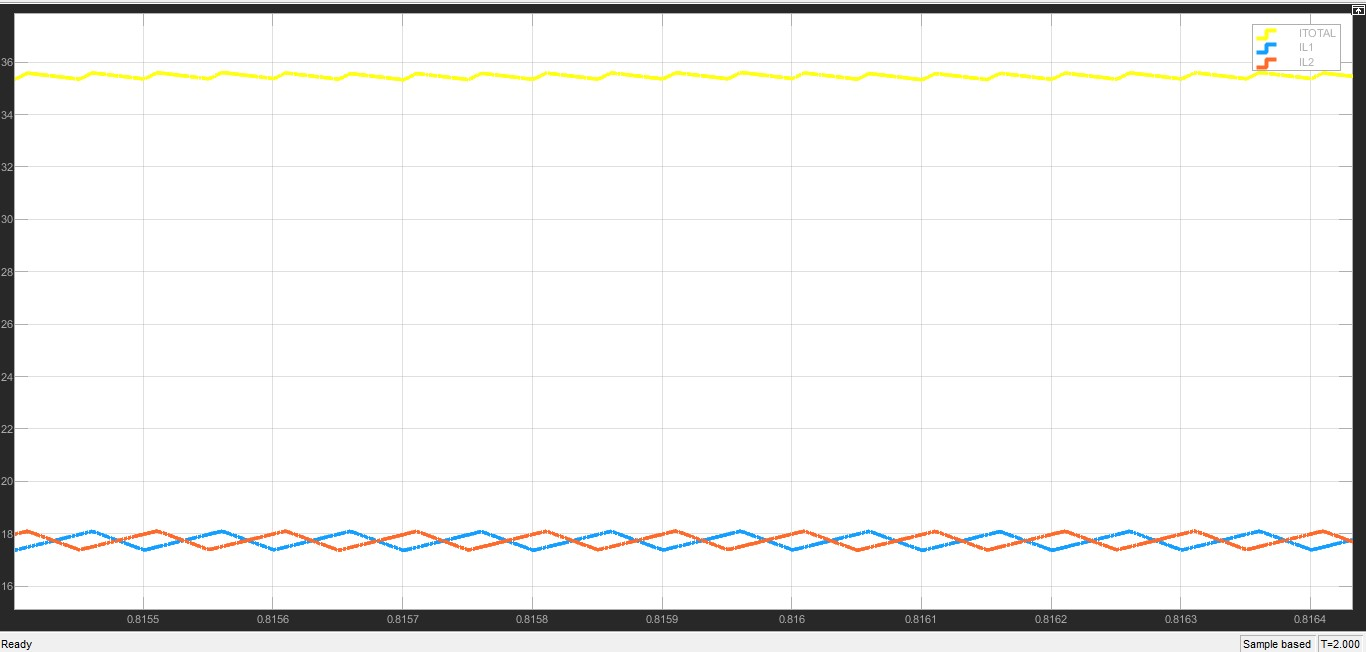
\includegraphics[width=0.85\textwidth]{Figures/case2/i2.jpg}
\caption{Zoomed View of the Interleaved Currents}
\label{fig:interleaved_zoom}
\end{figure}

The interleaved currents effectively regulate the power transfer from the ESS to the DC bus. The waveforms verify that the interleaving strategy remains stable while operating in Boost mode.

%%%%%%%%%%%%%%%%%%%%%%%%%%%%%%%%%%%%%%%%%%%%%%%%%%%%%%%%%%

\begin{figure}[H]
\centering
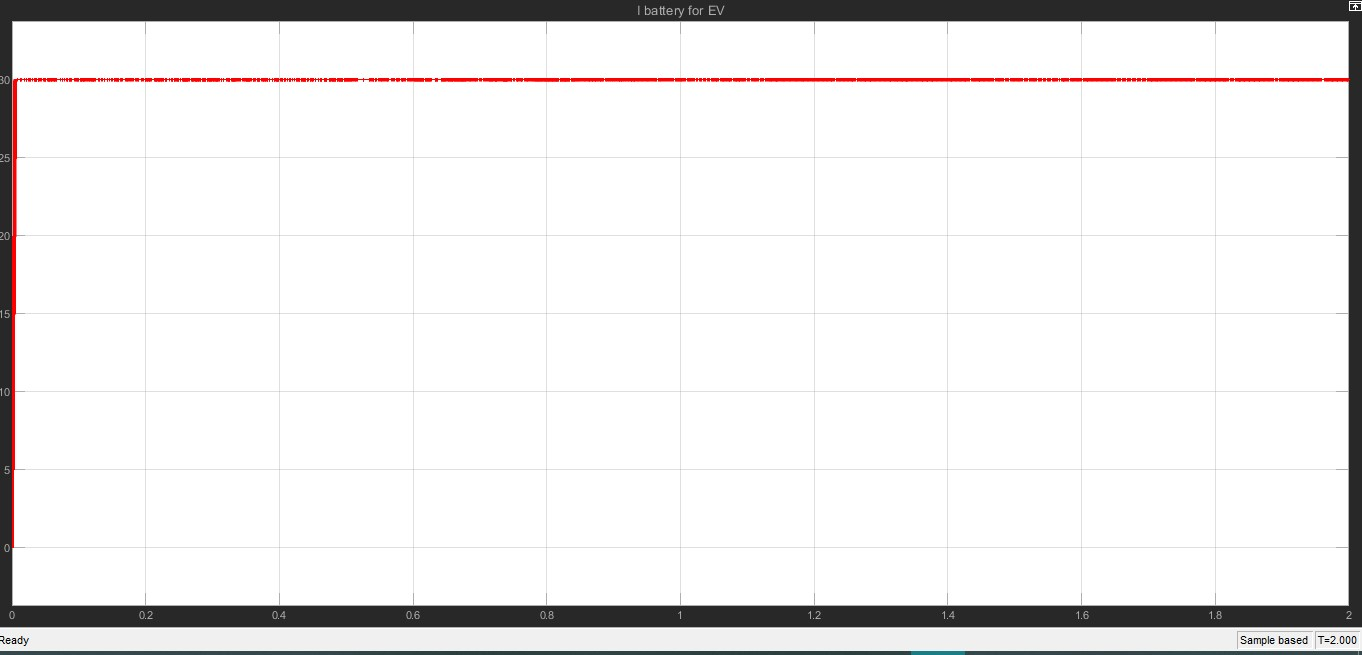
\includegraphics[width=0.85\textwidth]{Figures/case2/ibev.jpg}
\caption{EV Battery Charging Current}
\label{fig:ev_current_case2}
\end{figure}

The hysteresis current controller successfully regulates the EV charging current at the desired value of 30 A, ensuring stable power delivery even when the PV generation is insufficient.

%%%%%%%%%%%%%%%%%%%%%%%%%%%%%%%%%%%%%%%%%%%%%%%%%%%%%%%%%%

\begin{figure}[H]
\centering
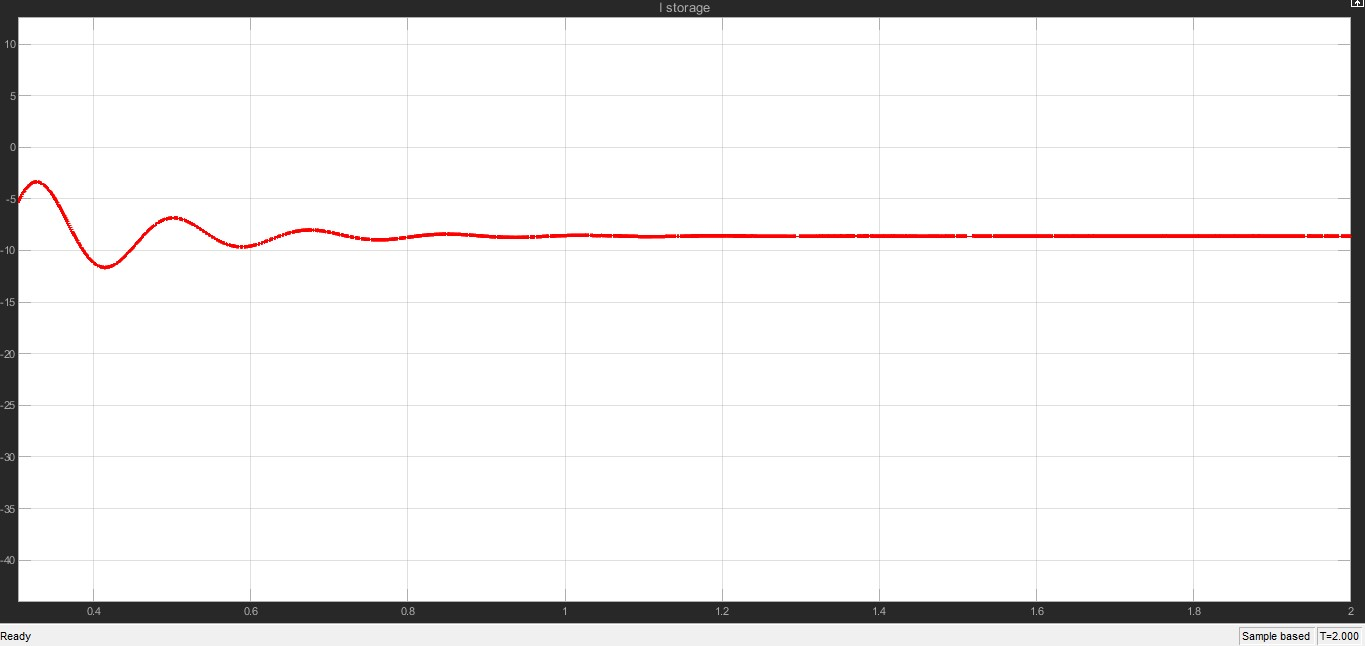
\includegraphics[width=0.85\textwidth]{Figures/case2/istorage.jpg}
\caption{ESS Discharge Current}
\label{fig:ess_discharge}
\end{figure}

The negative battery current indicates that the Energy Storage System is discharging and supplying approximately 3480 W to compensate for the deficit between the PV generation and the EV load demand.

%%%%%%%%%%%%%%%%%%%%%%%%%%%%%%%%%%%%%%%%%%%%%%%%%%%%%%%%%%

\begin{figure}[H]
\centering
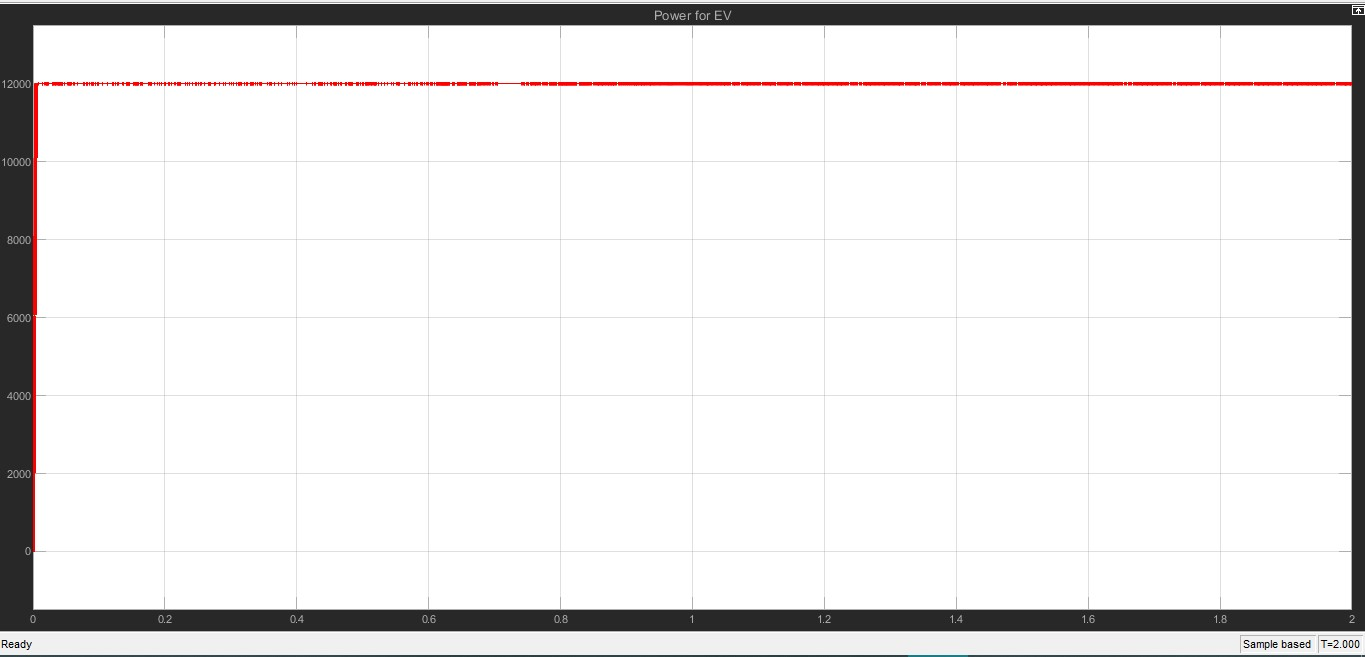
\includegraphics[width=0.85\textwidth]{Figures/case2/pev.jpg}
\caption{EV Load Power}
\label{fig:ev_power_case2}
\end{figure}

The EV load continuously receives the required 12 kW, demonstrating the capability of the proposed system to satisfy high load demand.

%%%%%%%%%%%%%%%%%%%%%%%%%%%%%%%%%%%%%%%%%%%%%%%%%%%%%%%%%%

\begin{figure}[H]
\centering
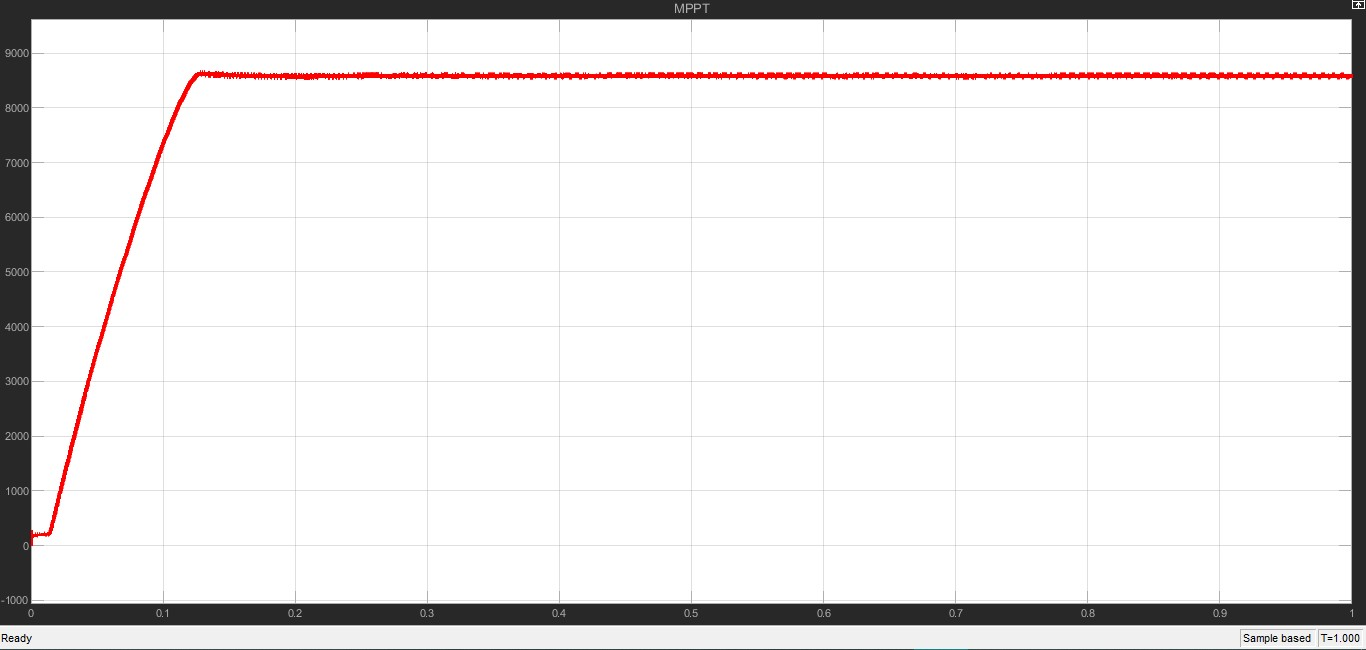
\includegraphics[width=0.85\textwidth]{Figures/pmppt.jpg}
\caption{PV Array Output Power}
\label{fig:pv_power_case2}
\end{figure}

The MPPT algorithm continuously tracks the maximum available power from the PV array and maintains an output power of approximately 8.52 kW.

%%%%%%%%%%%%%%%%%%%%%%%%%%%%%%%%%%%%%%%%%%%%%%%%%%%%%%%%%%

\begin{figure}[H]
\centering
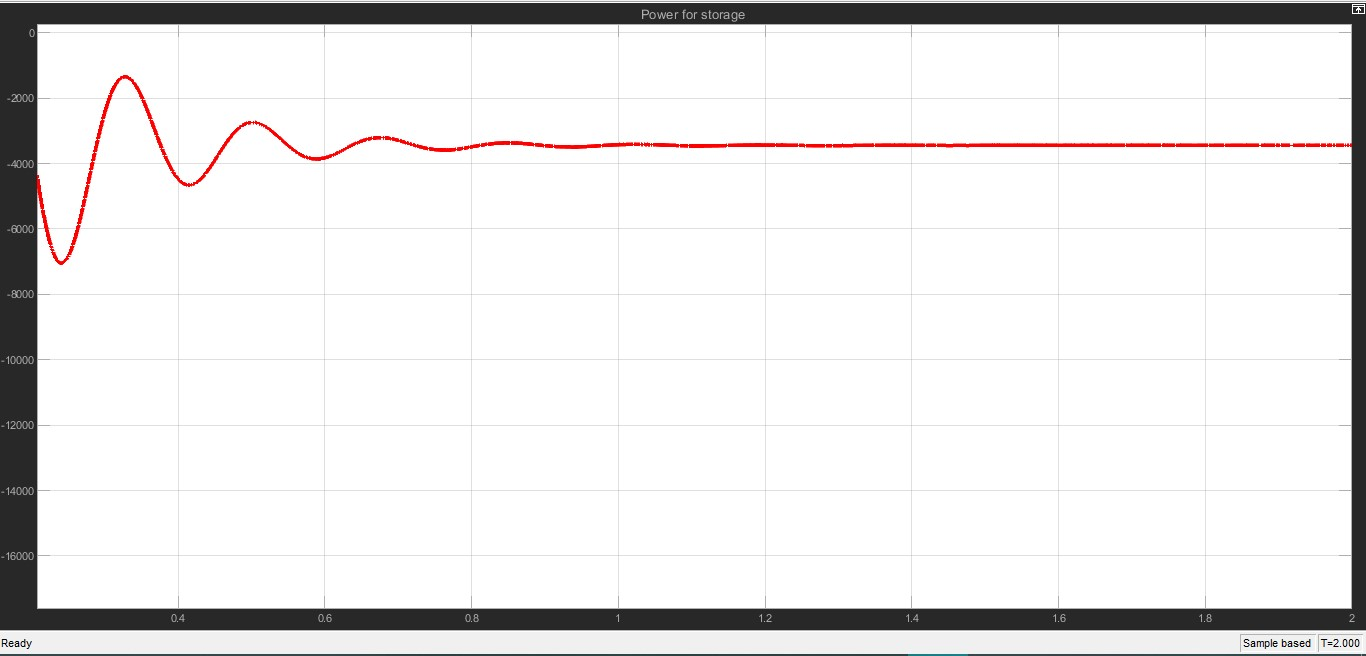
\includegraphics[width=0.85\textwidth]{Figures/case2/pstorage.jpg}
\caption{ESS Power Flow}
\label{fig:ess_power_case2}
\end{figure}

The waveform confirms that approximately 3480 W is delivered from the ESS to the DC bus, maintaining the required system power balance.

%%%%%%%%%%%%%%%%%%%%%%%%%%%%%%%%%%%%%%%%%%%%%%%%%%%%%%%%%%

\begin{figure}[H]
\centering
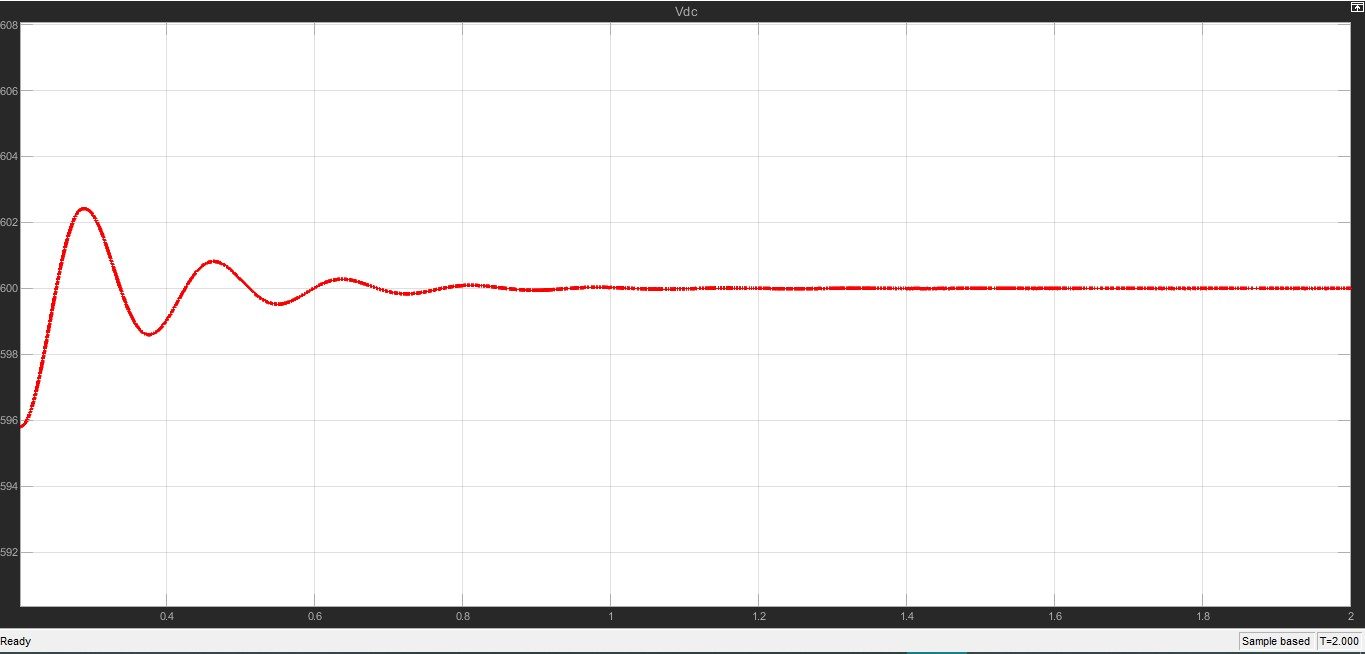
\includegraphics[width=0.85\textwidth]{Figures/case2/vdc.jpg}
\caption{DC Bus Voltage}
\label{fig:dcbus_case2}
\end{figure}

The DC bus voltage remains tightly regulated around 600 V throughout the Boost mode operation, confirming the effectiveness of the proposed control strategy.

%%%%%%%%%%%%%%%%%%%%%%%%%%%%%%%%%%%%%%%%%%%%%%%%%%%%%%%%%%

\begin{figure}[H]
\centering
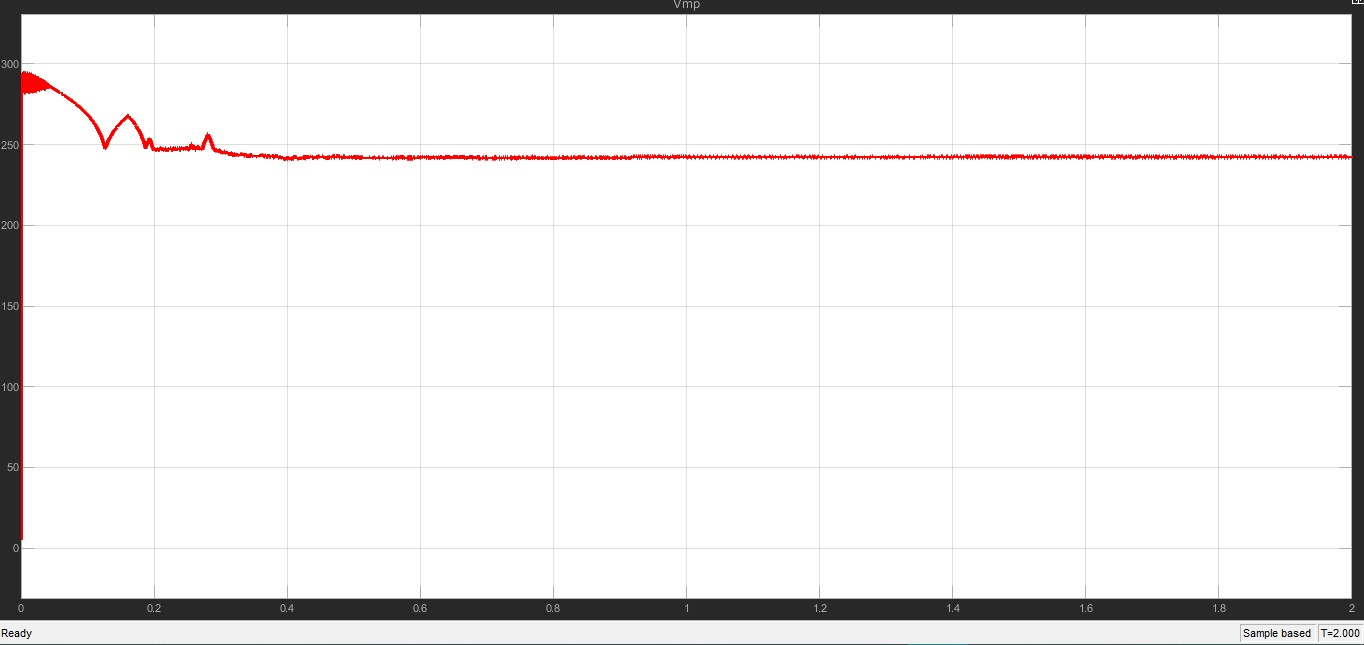
\includegraphics[width=0.85\textwidth]{Figures/case2/vmpt.jpg}
\caption{PV Voltage at the Maximum Power Point}
\label{fig:pv_voltage_case2}
\end{figure}

The PV voltage remains close to the maximum power point voltage, demonstrating accurate MPPT tracking and efficient utilization of the available solar energy.

\end{itemize}